\chapter{Adaptive LES of Flow Over Surging Airfoil}

In this chapter, we focus on applying the mesh adaptation strategies based on the VMS-based estimated error to large eddy simulation of flow over surging airfoil. A brief overview of the three strategies considered is mentioned in chapter \ref{sec:adapt_strat_overview}.

\section{Problem Setup}

The problem setup for these cases is similar to the one mentioned in Chapter \ref{sec:problem_setup_baseline}.

\section{Summary of Cases}

In this chapter, flow over a surging NACA 0012 airfoil is considered for $Re=40,000$ and $200,000$, for a sectional advance ratio of $\mu_{sect}=1.2$

\begin{table}[H]
	\centering
	\caption{Summary of cases}
	\label{table:summary_cases}
	\begin{tabular}{|l|c|c|c|c|}
		\hline
		Airfoil   & $\alpha$ & $k$ & $\mu_{sect}$ & $Re$ \\
		\hline
		\hline
		NACA 0012 & 6$^\circ$ & $0.133$ &  1.2 & 40,000\\
		\hline
		NACA 0012 & 6$^\circ$ & $0.133$ & 1.2 & 200,000 \\
	\hline
	\end{tabular}
\end{table}


Next, adaptive LES is performed for $Re=40,000$ and $Re=200,000$ cases, where a series of adapted meshes is constructed, and mesh convergence is shown.

\section{Comparison of Adaptive Strategies}
\label{sec:adaptive_strategy_comparison}
Here, a comparison of adaptive strategies is performed for the $Re=40,000$ case.%, at advance ratio of $\mu_{sect}=1.2$, at an angle of attack of $\alpha=6^\circ$.
The three VMS-based error estimator driven mesh adaptation strategies considered here are zonal-based refinement, nodal size field-based adaptation, and feature-based refinement.

\subsection{Zonal Refinement}
In this strategy, an initial solution is obtained on an initial mesh with a set of canonical refinement zones that are usually used for a flow over an airfoil. We refer to this mesh as M0\_nz25, see Figure \ref{fig:M0_mesh}. In-plane mesh sizes are indicated in the figure. The initial mesh spacing/resolution on the surface of the airfoil in the streamwise and spanwise directions is set to be below 75 and 40 in wall units, respectively.
Here nz25 refers to the number of spanwise extruded layers (i.e., 25) used in this mesh. 
As mentioned before, the VMS-based error estimator is applied to phase-averaged data, and the maximum error value over multiple phases (i.e., at 24 equispaced phases over the surging cycle), and over the spanwise direction, is selected to represent the element-level local error within the airfoil plane/section throughout the surging cycle. 
The element-level error estimated on this mesh is shown in Figure \ref{fig:M0_err_plot}. 
We can see that higher errors are observed primarily in the regions traversed by the LEV through the surging cycle, as well as in the wake of the airfoil. 
Higher errors are also observed close to the airfoil surface and in the boundary layer region.

Based on the estimated error, the mesh is refined by a factor of 2 in zones where high error values are found, including in the boundary layer mesh (i.e., along the streamwise direction). 
The spanwise resolution is also refined by a factor of 2 (i.e., the number of layers in the spanwise direction is doubled). 
This adapted mesh is shown in Figure \ref{fig:Mza1_mesh} and the estimated error on it is shown in Figure \ref{fig:Mza1_err_plot}. It is referred to as the Mza1\_nz50 mesh (where za is short for zonal adaptation and 1 in za1 denotes the first iteration of mesh adaptation).
%It is observed that the error has approximately reduced by a factor of 4 in the Mza1\_nz50 mesh as compared to the M0 mesh.
It is observed that the error has reduced in the Mza1\_nz50 mesh as compared to the M0 mesh
These meshes, M0\_nz25 and Mza1\_nz50, consist of 774,525 and 2,874,300 elements, respectively.

%Zonal refinements are added to the Mza1 mesh in regions of high error, and the mesh is refined further by a factor of 2 in these zones, along with the boundary layer mesh in the streamwise direction, and the number of layers in the spanwise direction is doubled.  This mesh, which is referred to as Mza2, is shown in Figure \ref{fig:Mza2_mesh}. Again, we observe that the error has reduced by a factor of 4 in the Mz\_a2 mesh as compared to Mz\_a1 mesh.

%The number of elements for each mesh is presented in Table \ref{table:mesh_zonal_summary}.


% \begin{table}[H]
% 	\centering
% 	\caption{Summary of zonal refinement based meshes}
% 	\label{table:mesh_zonal_summary}
% 	\begin{tabular}{|l|c|c|c|c|c|}
% 		\hline
% 		Mesh case  & No. of elements\\
% 		\hline
% 		\hline
% 		M0\_nz25 & 774,525 \\
% 		\hline
% 		Mza1\_nz50 &  2,874,300 \\
% 		\hline
% %		Mz\_a2 & 14,329,200 \\
% %		\hline
% 	\end{tabular}
	
% \end{table}

A comparison of different adaptive strategies/adapted meshes is provided in Section \ref{sec:results_adapt}.

\begin{figure}[H]
\centering
\begin{subfigure}[b]{0.475\textwidth}
\centering
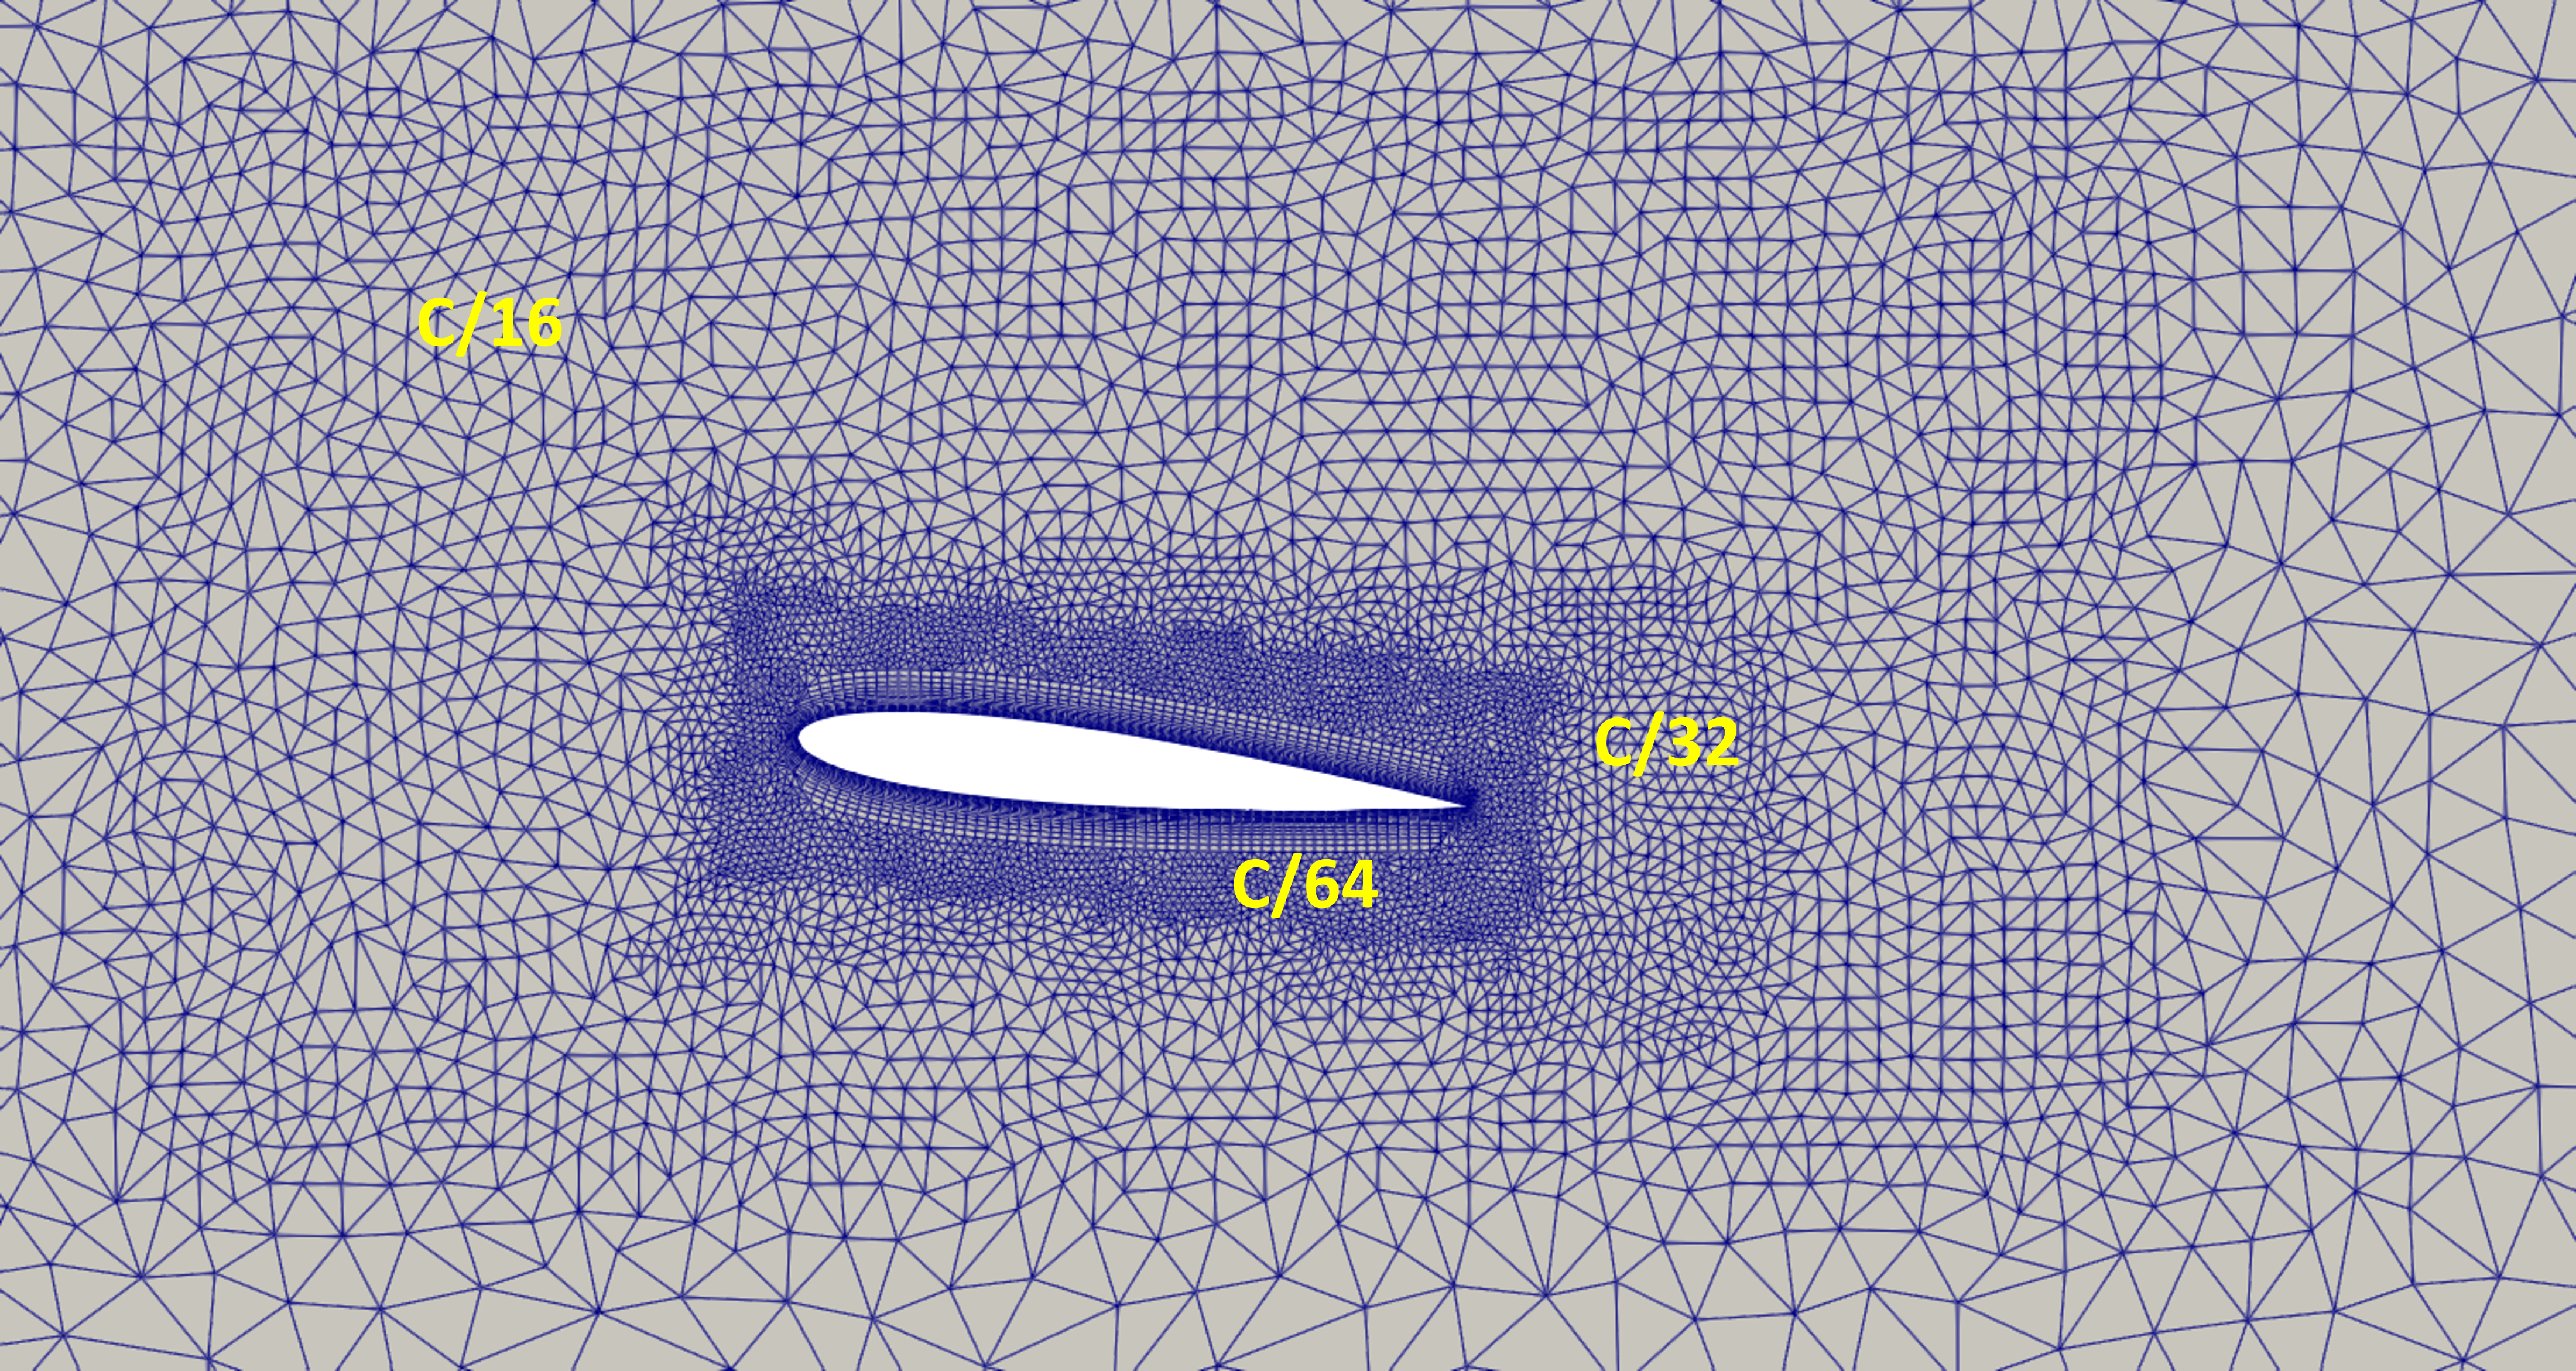
\includegraphics[width=1\textwidth]{figures/adapt_strat/M0_mesh.png}
\caption{M0\_nz25 mesh}
\label{fig:M0_mesh}
\end{subfigure}
\begin{subfigure}[b]{0.475\textwidth}
\centering
\includegraphics[width=1\textwidth]{figures/adapt_strat/M0_error.png}
\caption{M0\_nz25 error field}
\label{fig:M0_err_plot}
\end{subfigure}
\begin{subfigure}[b]{0.475\textwidth}
\centering
\includegraphics[width=1\textwidth]{figures/adapt_strat/Mza1_mesh.png}
\caption{Mza1\_nz50 mesh}
\label{fig:Mza1_mesh}
\end{subfigure}
\begin{subfigure}[b]{0.475\textwidth}
\centering
\includegraphics[width=1\textwidth]{figures/adapt_strat/Mza1_error.png}
\caption{Mza1\_nz50 error field}
\label{fig:Mza1_err_plot}
\end{subfigure}
%\begin{subfigure}[b]{0.475\textwidth}
%\centering
%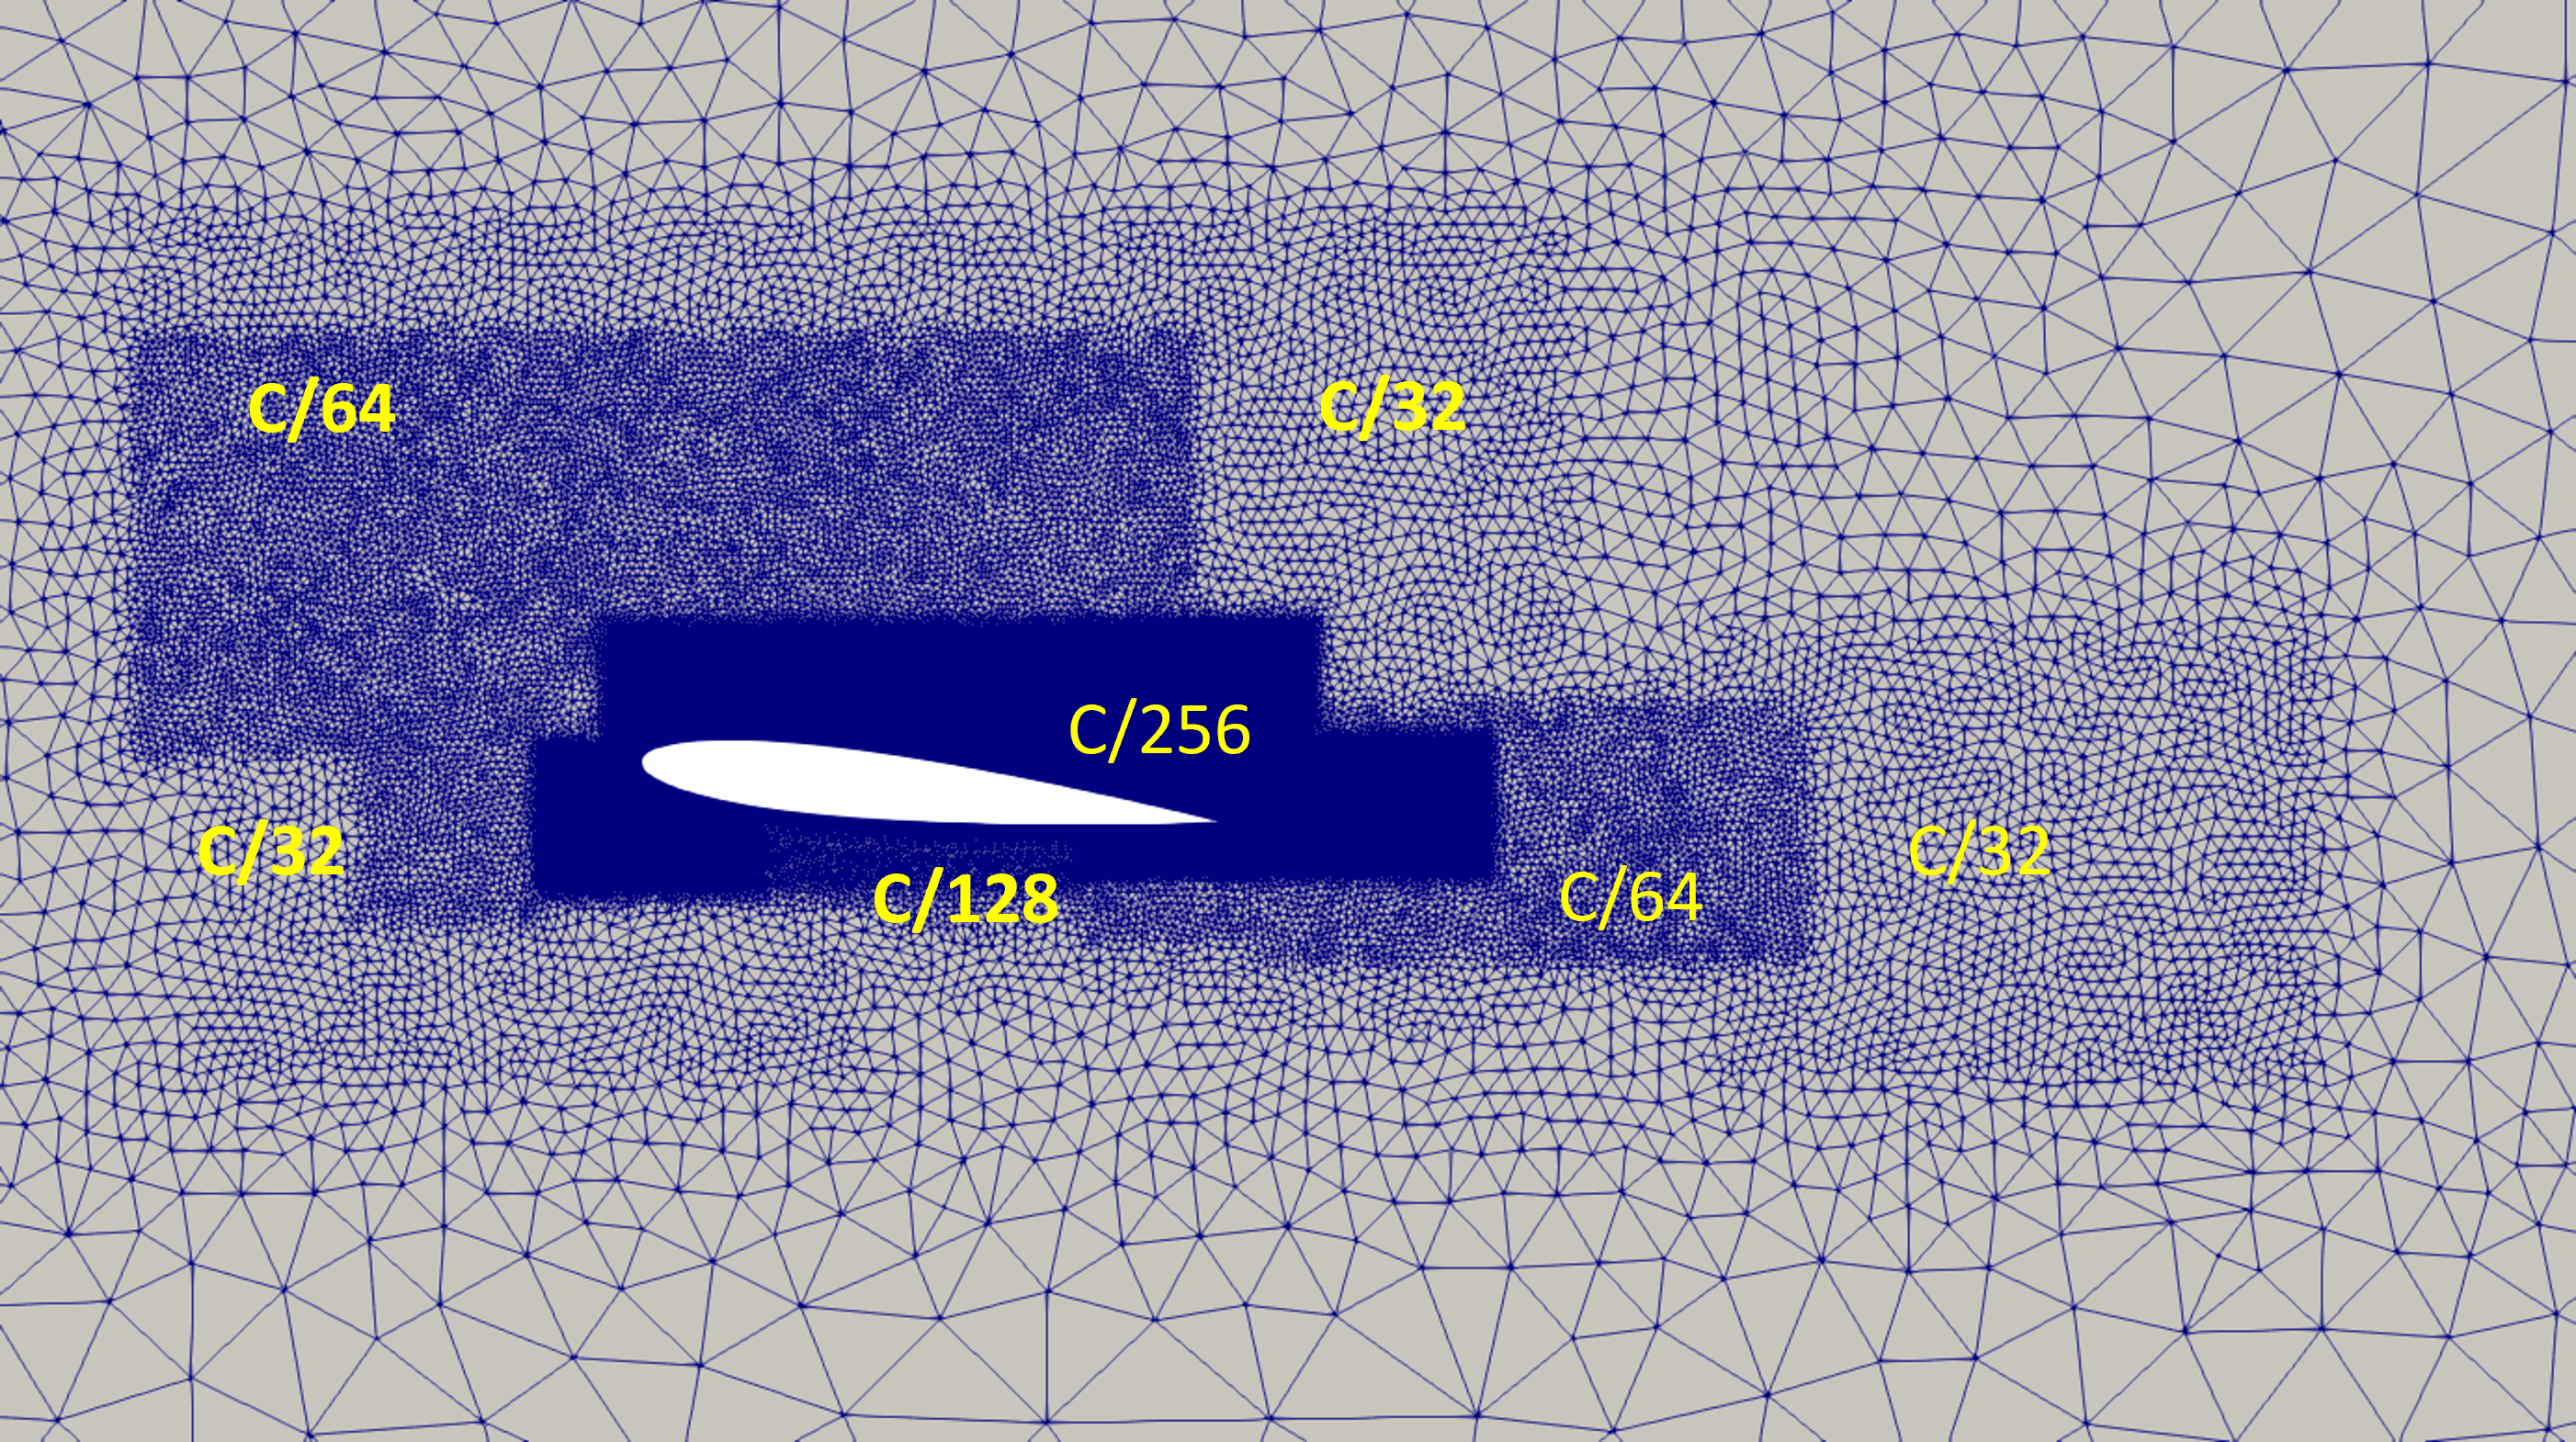
\includegraphics[width=1\textwidth]{figures/adapt_strat/Mza2_mesh.png}
%\caption{Mz\_a2 mesh}
%\label{fig:Mza2_mesh}
%\end{subfigure}
%\begin{subfigure}[b]{0.475\textwidth}
%\centering
%\includegraphics[width=1\textwidth]{figures/adapt_strat/Mza2_error_plot.png}
%\caption{Mz\_a2 error field}
%\label{fig:Mza2_err_plot}
%\end{subfigure}
\caption{Meshes and estimated error fields for zonal-based strategy}
\end{figure}



\subsection{Nodal Size Field-based Adaptation}
In this adaptive strategy, the VMS-based error is calculated on the initial mesh. Based on the estimated error, a nodal size field is calculated using the Equation \eqref{eq:diez}, see Section \ref{sec:sf_adapt}.

% \begin{equation}
% \frac{e_k}{\tilde{e}_k} = \left(\frac{h_{old}}{h_{new}}\right)^{m+N/2} 
% \label{eq:diez}
% \end{equation}

%Here, $e_k$ is the measured local error (in the $\HOne$-seminorm) at an element $k$, $\tilde{e}_k$ is the target error for an element specified by the user, $m$ is the polynomial order of the approximation space (i.e., $m=1$ for the linear finite elements used currently) , and $N$ is the number of spatial dimensions. $h_{old}$ is current size of the element, and $h_{new}$ is the desired new mesh size.
%This new mesh size at the element level is assembled at the node/vertex level to perform mesh adaptation.

\begin{figure}[H]
\centering
\begin{subfigure}[b]{0.475\textwidth}
\centering
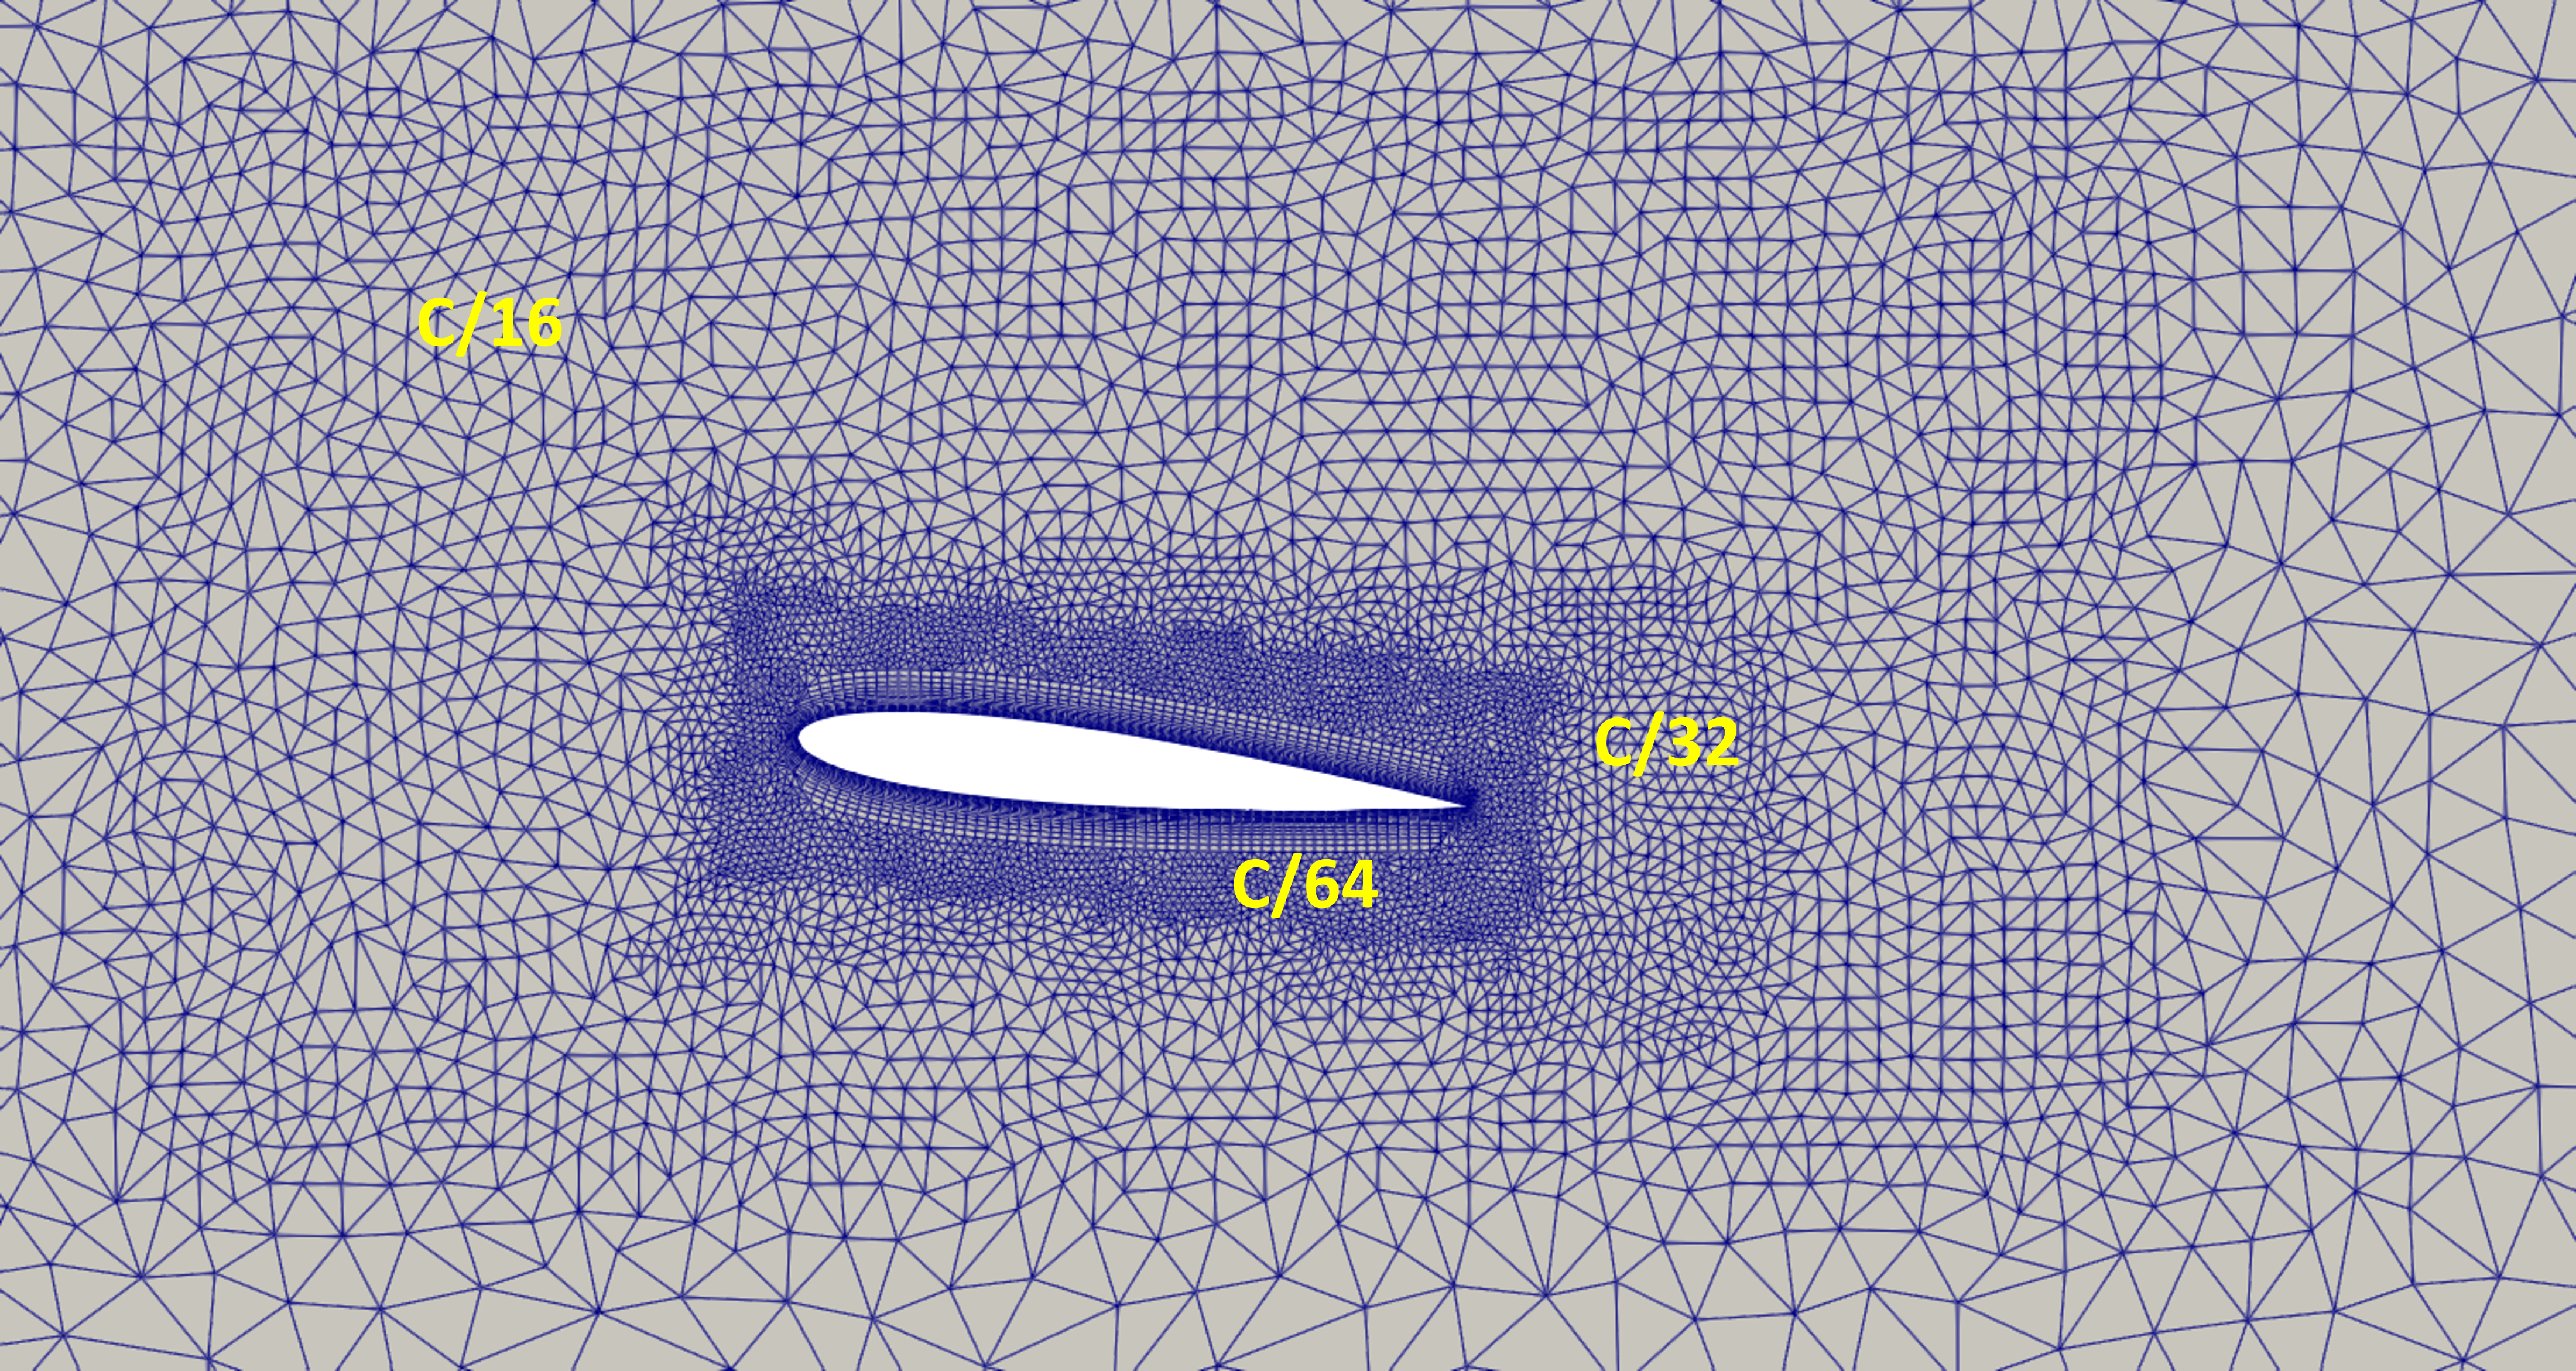
\includegraphics[width=1\textwidth]{figures/adapt_strat/M0_mesh.png}
\caption{M0\_nz25 mesh}
\label{fig:M0_mesh_sa}
\end{subfigure}
\begin{subfigure}[b]{0.475\textwidth}
\centering
\includegraphics[width=1\textwidth]{figures/adapt_strat/M0_error.png}
\caption{M0\_nz25 error field}
\label{fig:M0_err_plot_sa}
\end{subfigure}
\begin{subfigure}[b]{0.475\textwidth}
\centering
\includegraphics[width=1\textwidth]{figures/adapt_strat/Msa1_mesh.png}
\caption{Msa1\_nz50 mesh}
\label{fig:h_adapt1_mesh}
\end{subfigure}
\begin{subfigure}[b]{0.475\textwidth}
\centering
\includegraphics[width=1\textwidth]{figures/adapt_strat/Msa1_error.png}
\caption{Msa1\_nz50 error field}
\label{fig:h_adapt1_error_plot}
\end{subfigure}

\caption{Meshes and estimated error fields for size-based strategy}
\end{figure}

As before, M0\_nz25 is used as the initial mesh (Figure \ref{fig:M0_mesh}) and the corresponding error estimated on M0\_nz25 mesh (Figure \ref{fig:M0_err_plot}) is used to calculate nodal size field (i.e., $h_{new}$ at every mesh node/vertex). The mesh adaptation is limited or controlled to have a maximum refinement and maximum coarsening by a factor of 2 to avoid excessive refinement or coarsening in any local region. The number of extruded layers in the spanwise direction are doubled to 50. The adapted mesh obtained using this strategy is shown in Figure \ref{fig:h_adapt1_mesh}. It is referred to as the Msa1\_nz50 mesh (where sa is short for size-based adaptation and 1 in sa1 denotes the first iteration of mesh adaptation). Note that in terms of mesh resolution, this adapted mesh, Msa1\_nz50, compares well against the Mza1\_nz50 mesh obtained from the zonal-based strategy. Msa1\_nz25 mesh consists of 2,859,450 elements, which is comparable to 2,874,300 elements for the Mza1\_n50 mesh. The major differences between the two meshes is that Mza1\_nz50 maintains the same mesh size in various zones, whereas mesh size varies locally (even within a zone) in Msa1\_nz50.
The corresponding estimated error for this mesh is shown in Figure \ref{fig:h_adapt1_error_plot}. M0\_nz0 mesh and error field are shown again to compare against Msa1\_nz50. Comparing the estimated error between the Msa1\_nz50 and Mza1\_nz50 meshes, higher error values are observed in the LEV regions as well as in the wake of the airfoil. Overall, the estimated error on the Msa1\_nz50 mesh is higher as compared to that on the Mza1\_nz50 mesh. A more detailed comparison of different adaptive strategies/adapted meshes is provided in Section \ref{sec:results_adapt}.


\subsection{Feature-based Refinement}
In this strategy, mesh refinement is applied around the dominant flow features of interest.
In the current surging airfoil case, LEV is the dominant flow feature. 
Using vortex detection and tracking (see Section \ref{sec:LEV_detect_track}), LEV evolution (path and size) is determined using an initial mesh (M0\_nz25 in this case). 
Based on this a refinement zone is added around the path of the LEV.
In such a feature-based refinement, VMS-based estimated error is used to set the mesh size in the refinement zone(s) around the dominant feature(s). 
In addition, estimated error is also used to refine the mesh around the airfoil (e.g., in a similar fashion as the error-based zonal refinement discussed earlier). 
This is done to accurately resolve the flow near the airfoil including the boundary layer region that plays a direct role in the formation of LEV.

In summary, the mesh around the LEV path is refined by a factor of 2. In addition, the boundary layer mesh is refined by a factor of 2 in the streamwise direction, and again, the number of layers in the spanwise direction are doubled as compared to M0\_nz25.
The resulting mesh resolution on the surface of the airfoil in the streamwise and spanwise directions is below 40 and 25 in wall units, respectively, i.e., same as the previous cases.
This adapted mesh is referred to as the Mfa1\_nz50 mesh (where fa is short for feature-based adaptation and 1 in fa1 denotes the first iteration of mesh adaptation). 
This mesh is shown in Figure \ref{fig:FB_mesh} and the estimated error on it is shown in Figure \ref{fig:FB_error_plot}.
M0\_nz0 mesh and error field are shown again to compare against Mfa1\_nz50.
Mfa1\_nz50 contains 2,777,750 elements, which is comparable to both Mza1\_nz50 and Msa1\_nz50 meshes.

Error values are similar to those obtained on the Mza1\_nz50 mesh, i.e., near the airfoil surface, in the LEV path, and in the wake, since mesh resolution in crucial regions is similar between the Mfa1\_nz50 and Mza1\_nz50 meshes, while estimated error is higher on the Msa1\_nz50 mesh.
%Error values are lower as compared to Msa1\_nz50, since a uniform mesh size is maintained, as opposed to Msa1\_nz50, where the mesh size is patchy.
A more detailed comparison of different adaptive strategies/adapted meshes is provided in Section \ref{sec:results_adapt}.

\begin{figure}[H]
\centering
\begin{subfigure}[b]{0.475\textwidth}
\centering
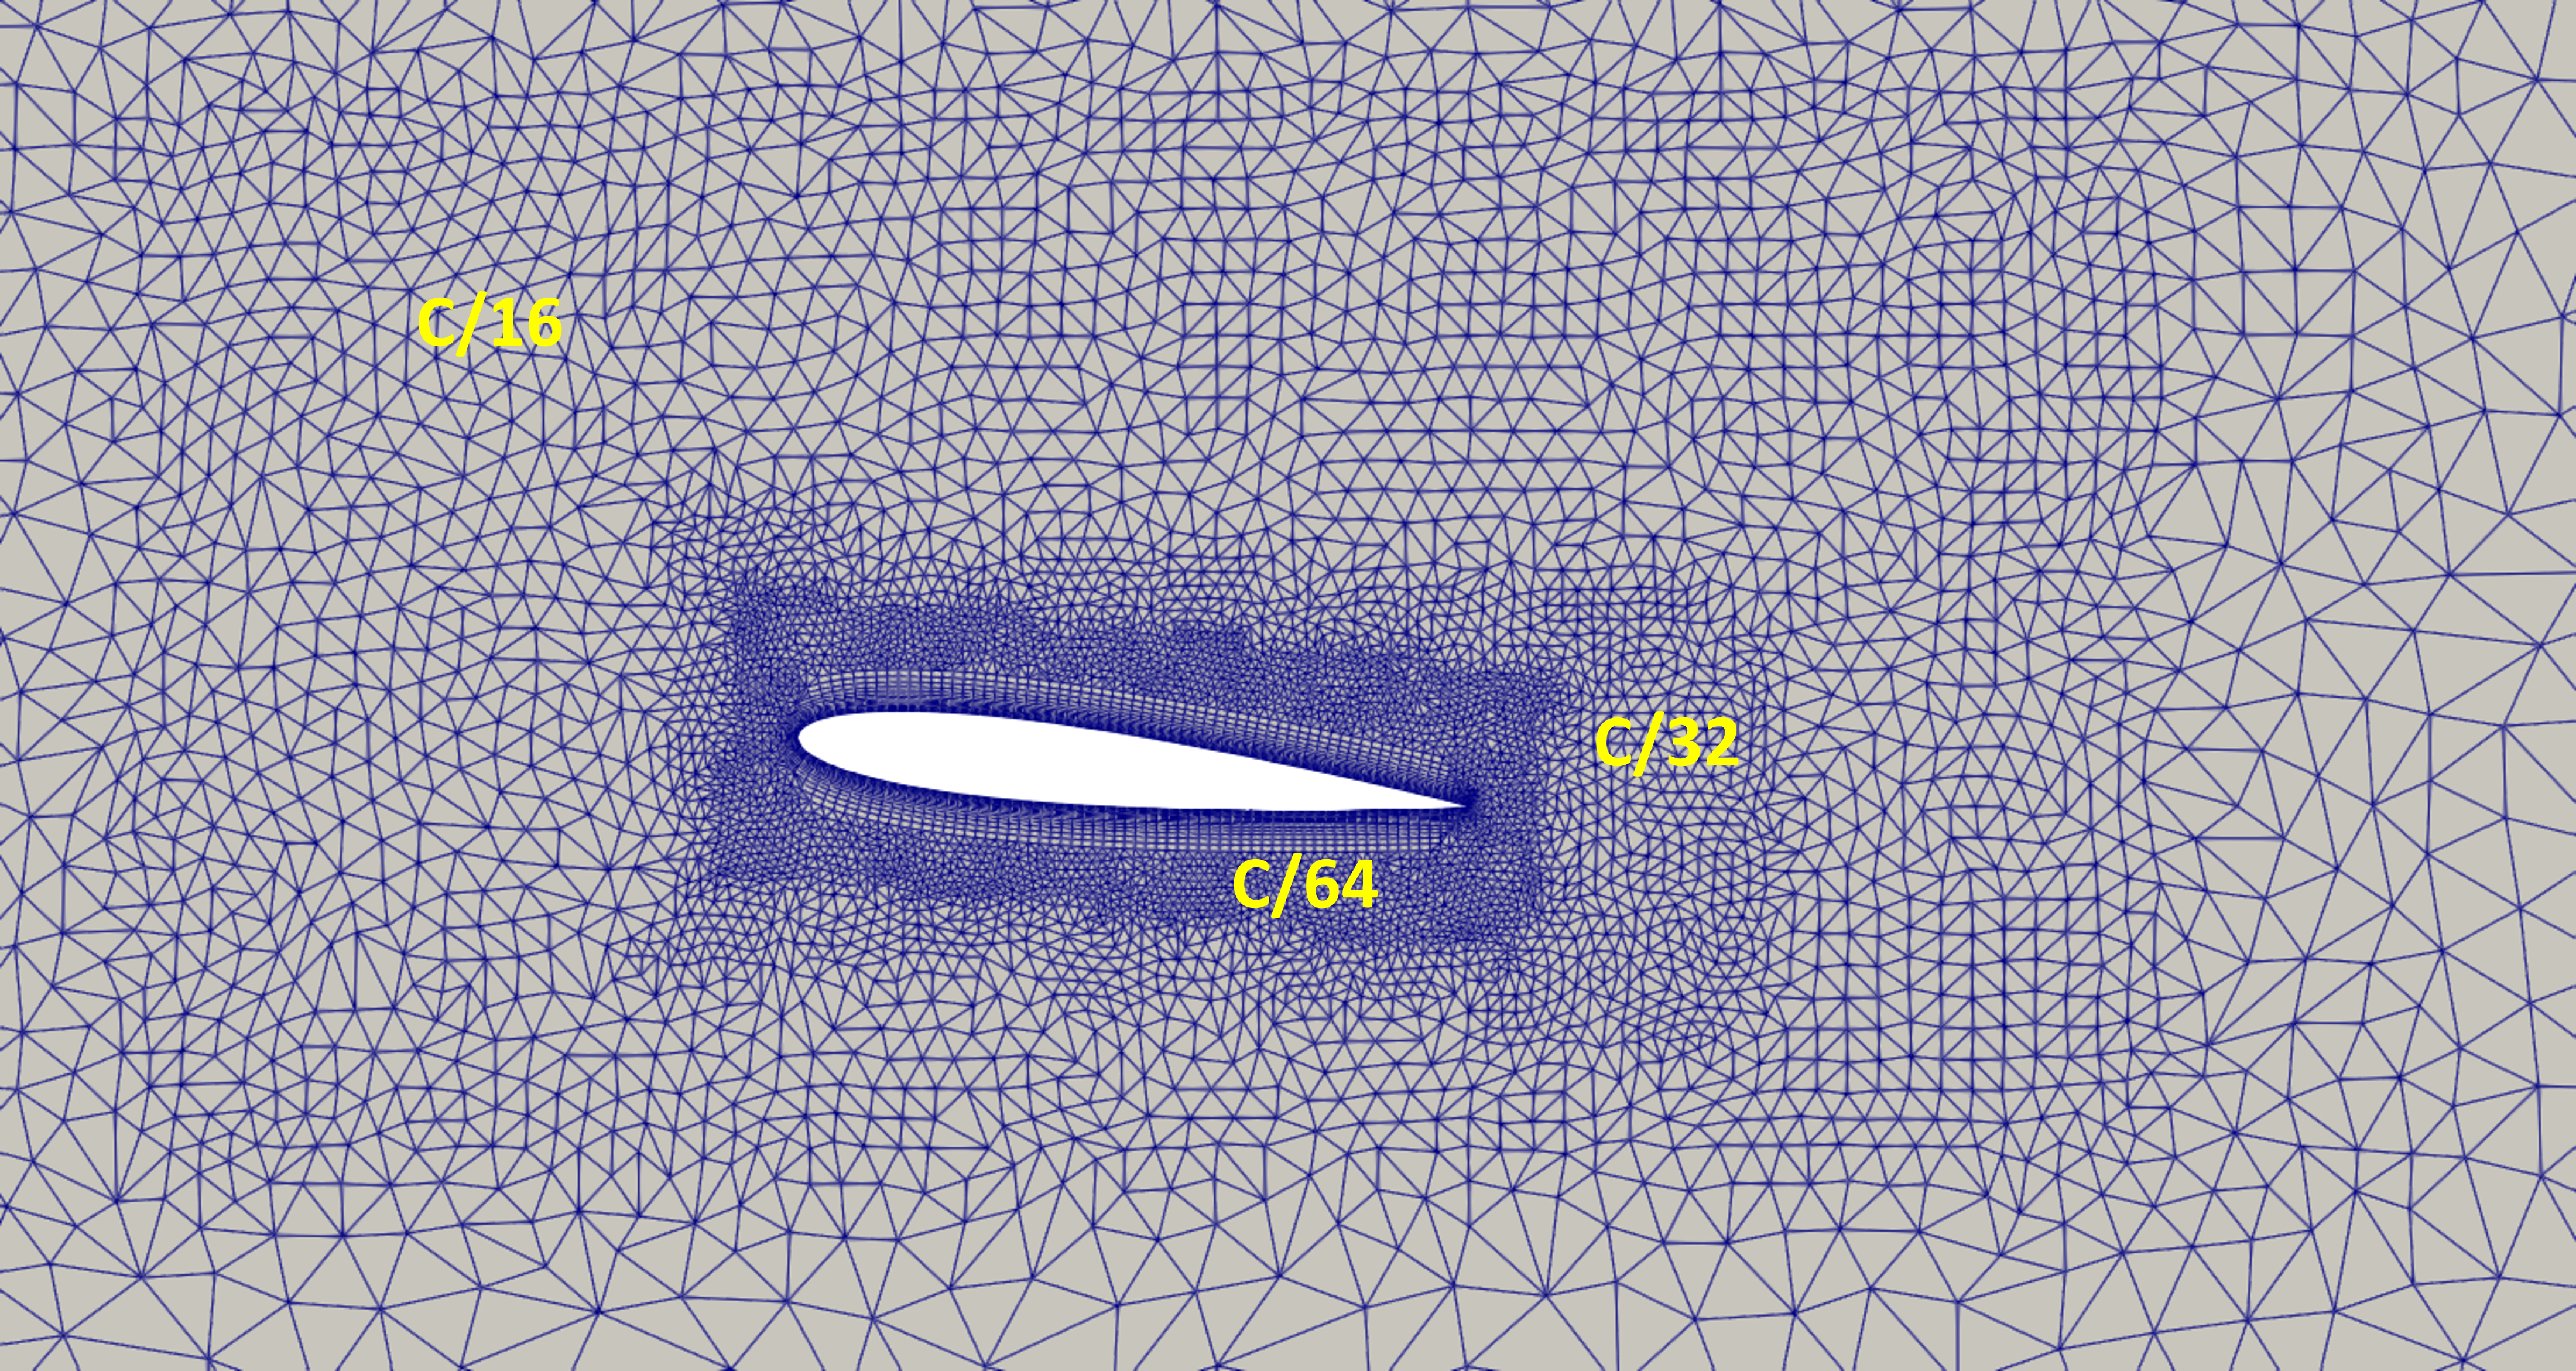
\includegraphics[width=1\textwidth]{figures/adapt_strat/M0_mesh.png}
\caption{M0\_nz25 mesh}
\label{fig:M0_mesh_fa}
\end{subfigure}
\begin{subfigure}[b]{0.475\textwidth}
\centering
\includegraphics[width=1\textwidth]{figures/adapt_strat/M0_error.png}
\caption{M0\_nz25 error field}
\label{fig:M0_err_plot_fa}
\end{subfigure}
\begin{subfigure}[b]{0.475\textwidth}
\centering
\includegraphics[width=1\textwidth]{figures/adapt_strat/Mfa1_mesh.png}
\caption{Mfa1\_nz50 mesh}
\label{fig:FB_mesh}
\end{subfigure}
\begin{subfigure}[b]{0.475\textwidth}
\centering
\includegraphics[width=1\textwidth]{figures/adapt_strat/Mfa1_error.png}
\caption{Mfa1\_nz50 error field}
\label{fig:FB_error_plot}
\end{subfigure}

\caption{Meshes and estimated error fields for feature-based strategy}
\end{figure}
\label{sec:feature_based_strat}


\subsection{Results and Discussion}
In this section, we compare results of different adapted meshes obtained from three adaptive strategies mentioned above. 
We compare different quantities of interest. 
A comparison of force response in the form of normalized lift and drag forces is shown in Figures \ref{fig:lift_plot} and \ref{fig:drag_plot}, respectively. The normalized lift and drag matches up well for all the adapted meshes.

A comparison of spanwise vorticity for the different adapted meshes is shown in Figures \ref{fig:vorticity_195}, \ref{fig:vorticity_210} and \ref{fig:vorticity_270}, for 3 phases of $\psi=210^\circ$, $\psi=225^\circ$ and $\psi=270^\circ$, respectively.
For $\psi=195^\circ$, as the airfoil is in the retreating phase, boundary layer roll-up towards the geometric leading edge is observed over the airfoil surface.
For the meshes based on zonal refinement, as we go from M0\_nz25 to Mza1\_nz50, the separation over the airfoil is well resolved, and finer scales or flow structures are visible on the adapted mesh.
Comparing Mza1\_nz50, Msa1\_nz50, and Mfa1\_nz50 meshes, we can see that the Msa1\_nz50 mesh (sizefield-based adapted mesh) does not capture the finer scales/structures as compared to the Mza1\_nz50 mesh, both over the airfoil surface and in the wake of the airfoil, i.e., flow structures are more diffused in the case of Msa1\_nz50.
On the other hand, the Mfa1\_nz50 mesh captures them well.

\begin{figure}[H]
\centering

\begin{subfigure}[b]{0.7\textwidth}
\centering
\includegraphics[width=1\textwidth]{figures/Results/Lift_adapt_strat.png}
\caption{Normalized lift}
\label{fig:lift_plot}
\end{subfigure}
\begin{subfigure}[b]{0.7\textwidth}
\centering
\includegraphics[width=1\textwidth]{figures/Results/Drag_adapt_strat.png}
\caption{Normalized drag}
\label{fig:drag_plot}
\end{subfigure}

\label{fig:force_response_adapt}
\caption{Normalized forces for different adaptive strategies/adapted meshes}
\end{figure}

%Next, we look at the location of the LEV core for different meshes in Figure \ref{fig:LEV_location}. Some differences in the LEV location for various phases are observed. LEV location for Ma1, FB, and hadapt meshes is similar in the beginning phases. Ma1 starts to deviate from FB and hadapt in the later phases. LEV location for FB and hadapt meshes start to match with Ma2 in the later phases, whereas M0 LEV location fluctuates around the other meshes. This however is still not conclusive as to which mesh performs better and a more quantitative study is needed.


%%\begin{figure}[H]
%\centering
%\includegraphics[width=0.7\textwidth]{figures/Results/LEV_location.png}
%\caption{LEV location for different meshes}
%\label{fig:LEV_location}
%\end{figure}
%%


For $\psi=210^\circ$, formation of LEV begins to take place, as we start to see the roll-up of separated shear layer near the geometric leading edge. 
At this phase, the differences in the structures resolved by the different meshes become more clear.
Similar to $\psi=195^\circ$, the Msa1\_nz50 mesh shows a relatively poor resolution of the finer flow structures as compared to the Mza1\_nz50 and Mfa1\_nz50 meshes.

For $\psi=270^\circ$, differences can be seen in the separated shear layer at the geometric leading edge of the airfoil, and the resolution of the LEV, among different adapted meshes.
These are resolved better on the Mfa1\_nz50 and Mza1\_nz50 meshes. 
Recall that Mfa1\_nz50 is obtained using feature-based mesh refinement designed to capture the LEV accurately, and has the same mesh resolution as Mza1\_nz50 along the path of the LEV. 
%Once again, shear layer is not well resolved for Msa1\_nz50 as compared to other refined/adapted meshes.

The relatively poor resolution of flow, with more diffused flow structures, observed for Msa1\_nz50 can be attributed to the variation in mesh sizes (even by a factor of 1.5 or 2) in crucial regions of interest, i.e., the mesh size is not uniform or even quasi-uniform in particular zones. In particular, this seem to have an adverse effect in regions with turbulence.

\begin{figure}[H]
\centering
\begin{subfigure}[b]{0.475\textwidth}
\centering
\includegraphics[width=1\textwidth]{figures/adapt_strat/vorticity_plots/M0/phase_195.png}
\caption{M0\_nz25 mesh, $\psi$ = $195^\circ$}
\label{fig:M0_psi195}
\end{subfigure}
\begin{subfigure}[b]{0.475\textwidth}
\centering
\includegraphics[width=1\textwidth]{figures/adapt_strat/vorticity_plots/Mza1_50/phase_195.png}
\caption{Mza1\_nz50 mesh, $\psi$ = $195^\circ$}
\label{fig:Ma1_psi195}
\end{subfigure}
%\begin{subfigure}[b]{0.475\textwidth}
%\centering
%\includegraphics[width=1.25\textwidth]{figures/vorticity_plots/Mza2/ph_195.png}
%\caption{Mz\_a2 mesh, $\psi$ = $195^\circ$}
%\label{fig:Ma2_psi195}
%\end{subfigure}
\begin{subfigure}[b]{0.475\textwidth}
\centering
\includegraphics[width=1\textwidth]{figures/adapt_strat/vorticity_plots/Msa1_50/phase_195.png}
\caption{Msa1\_nz50 mesh, $\psi$ = $195^\circ$}
\label{fig:hadapt_psi195}
\end{subfigure}
\begin{subfigure}[b]{0.475\textwidth}
\centering
\includegraphics[width=1\textwidth]{figures/adapt_strat/vorticity_plots/Mfa1_50/phase_195.png}
\caption{Mfa1\_nz50 mesh, $\psi$ = $195^\circ$}
\label{fig:FB_psi195}
\end{subfigure}
\caption{Spanwise vorticity comparison at $\psi$ = $195^\circ$ for different adaptive strategies/adapted meshes}
\label{fig:vorticity_195}
\end{figure}



\begin{figure}[H]
\centering
\begin{subfigure}[b]{0.475\textwidth}
\centering
\includegraphics[width=1\textwidth]{figures/adapt_strat/vorticity_plots/M0/phase_210.png}
\caption{M0\_nz25 mesh, $\psi$ = $210^\circ$}
\label{fig:M0_psi210}
\end{subfigure}
\begin{subfigure}[b]{0.475\textwidth}
\centering
\includegraphics[width=1\textwidth]{figures/adapt_strat/vorticity_plots/Mza1_50/phase_210.png}
\caption{Mza1\_nz50 mesh, $\psi$ = $210^\circ$}
\label{fig:Mza1_psi210}
\end{subfigure}
%\begin{subfigure}[b]{0.475\textwidth}
%\centering
%\includegraphics[width=1.25\textwidth]{figures/vorticity_plots/Mza2/ph_210.png}
%\caption{Mz\_a2 mesh, $\psi$ = $210^\circ$}
%\label{fig:Ma2_psi210}
%\end{subfigure}
\begin{subfigure}[b]{0.475\textwidth}
\centering
\includegraphics[width=1\textwidth]{figures/adapt_strat/vorticity_plots/Msa1_50/phase_210.png}
\caption{Msa1\_nz50 mesh, $\psi$ = $210^\circ$}
\label{fig:hadapt_psi210}
\end{subfigure}
\begin{subfigure}[b]{0.475\textwidth}
\centering
\includegraphics[width=1\textwidth]{figures/adapt_strat/vorticity_plots/Mfa1_50/phase_210.png}
\caption{Mfa1\_nz50 mesh, $\psi$ = $210^\circ$}
\label{fig:FB_psi210}
\end{subfigure}
\caption{Spanwise vorticity comparison at $\psi$ = $210^\circ$ for different adaptive strategies/adapted meshes}
\label{fig:vorticity_210}
\end{figure}



%%VORTICITY PLOT
\begin{figure}[H]
\centering

\begin{subfigure}[b]{0.475\textwidth}
\centering
\includegraphics[width=1\textwidth]{figures/adapt_strat/vorticity_plots/M0/phase_270.png}
\caption{M0\_nz25 mesh, $\psi$ = $270^\circ$}
\label{fig:M0_psi270}
\end{subfigure}
\begin{subfigure}[b]{0.475\textwidth}
\centering
\includegraphics[width=1\textwidth]{figures/adapt_strat/vorticity_plots/Mza1_50/phase_270.png}
\caption{Mza1\_nz50 mesh, $\psi$ = $270^\circ$}
\label{fig:Ma1_psi270}
\end{subfigure}
%\begin{subfigure}[b]{0.475\textwidth}
%\centering
%\includegraphics[width=1.25\textwidth]{figures/vorticity_plots/Mza2/ph_270.png}
%\caption{Mz\_a2 mesh, $\psi$ = $270^\circ$}
%\label{fig:Ma2_psi270}
%\end{subfigure}
\begin{subfigure}[b]{0.475\textwidth}
\centering
\includegraphics[width=1\textwidth]{figures/adapt_strat/vorticity_plots/Msa1_50/phase_270.png}
\caption{Msa1\_nz50 mesh, $\psi$ = $270^\circ$}
\label{fig:hadapt_psi270}
\end{subfigure}
\begin{subfigure}[b]{0.475\textwidth}
\centering
\includegraphics[width=1\textwidth]{figures/adapt_strat/vorticity_plots/Mfa1_50/phase_270.png}
\caption{Mfa1\_nz50 mesh, $\psi$ = $270^\circ$}
\label{fig:FB_psi270}
\end{subfigure}
\caption{Spanwise vorticity comparison at $\psi$ = $270^\circ$ for different adaptive strategies/adapted meshes}
\label{fig:vorticity_270}
\end{figure}

Figures \ref{fig:Mza1_zoomed}, \ref{fig:Msa1_zoomed} and \ref{fig:Mfa1_zoomed} show a zoomed-in view of the mesh, spanwise vorticity at $\psi=210^\circ$, and the element-level/local error (maximum over multiple phases and over the spanwise direction). This is done for Mza1\_nz50, Msa1\_nz50, and Mfa1\_nz50 meshes.
The different meshes in these figures show that a quasi-uniform mesh size is maintained in specified zones for both Mza1\_nz50 and Mfa1\_nz50, while the Msa1\_nz50 mesh is patchy, i.e., a uniform mesh size is not maintained in Msa1\_nz50.
The error field for Msa1\_nz50 is also patchy, as compared to Mza1\_nz50 and Mfa1\_nz50, with elements that have a higher local estimated error in Msa1\_nz50.
This becomes further evident from the vorticity plots, especially in the wake region, where Msa1\_nz50 shows a poor resolution of fine-scale flow structures, as compared to Mza1\_nz50 and Mfa1\_nz50.
Note that the Mza1\_nz50 and Mfa1\_nz50 meshes are very comparable and the zonal refinement encompasses the regions/portions covered by the feature/LEV-based refinement, and thus, they turn out to be equivalent for the current case.

\begin{figure}[H]
	\centering
\begin{subfigure}[b]{0.7\textwidth}
	\centering
	\includegraphics[width=1\textwidth]{figures/adapt_strat/zoomed/Mza1_mesh.png}
	\caption{Mza1\_nz50 mesh}
	\label{fig:Mza1_mesh_zoomed}
\end{subfigure}
\begin{subfigure}[b]{0.7\textwidth}
	\centering
	\includegraphics[width=1\textwidth]{figures/adapt_strat/zoomed/Mza1_error.png}
	\caption{Mza1\_nz50 estimated error}
	\label{fig:Mza1_max_error_zoomed}
\end{subfigure}
\begin{subfigure}[b]{0.7\textwidth}
	\centering
	\includegraphics[width=1\textwidth]{figures/adapt_strat/zoomed/Mza1_ph_210.png}
	\caption{Mza1\_nz50 vorticity at $\psi=210^\circ$}
	\label{fig:Mza1_vorticity_zoomed}
\end{subfigure}
\caption{Zoomed-in view for Mza1\_nz50: mesh, estimated error and vorticity}
\label{fig:Mza1_zoomed}
\end{figure}

\begin{figure}[H]
	\centering
	\begin{subfigure}[b]{0.7\textwidth}
		\centering
		\includegraphics[width=1\textwidth]{figures/adapt_strat/zoomed/Msa1_mesh.png}
		\caption{Msa1\_nz50 mesh}
		\label{fig:Msa1_mesh_zoomed}
	\end{subfigure}
	\begin{subfigure}[b]{0.7\textwidth}
		\centering
		\includegraphics[width=1\textwidth]{figures/adapt_strat/zoomed/Msa1_error.png}
		\caption{Msa1\_nz50 estimated error}
		\label{fig:Msa1_max_error_zoomed}
	\end{subfigure}
	\begin{subfigure}[b]{0.7\textwidth}
		\centering
		\includegraphics[width=1\textwidth]{figures/adapt_strat/zoomed/Msa1_ph_210.png}
		\caption{Msa1\_nz50 vorticity at $\psi=210^\circ$}
		\label{fig:Msa1_vorticity_zoomed}
	\end{subfigure}
	\caption{Zoomed-in view for Msa1\_nz50: mesh, estimated error and vorticity}
	\label{fig:Msa1_zoomed}
\end{figure}


\begin{figure}[H]
	\centering
	\begin{subfigure}[b]{0.7\textwidth}
		\centering
		\includegraphics[width=1\textwidth]{figures/adapt_strat/zoomed/Mfa1_mesh.png}
		\caption{Mfa1\_nz50 mesh}
		\label{fig:Mfa1_mesh_zoomed}
	\end{subfigure}
	\begin{subfigure}[b]{0.7\textwidth}
		\centering
		\includegraphics[width=1\textwidth]{figures/adapt_strat/zoomed/Mfa1_error.png}
		\caption{Mfa1\_nz50 estimated error}
		\label{fig:Mfa1_max_error_zoomed}
	\end{subfigure}
	\begin{subfigure}[b]{0.7\textwidth}
		\centering
		\includegraphics[width=1\textwidth]{figures/adapt_strat/zoomed/Mfa1_ph_210.png}
		\caption{Mfa1\_nz50 vorticity at $\psi=210^\circ$}
		\label{fig:Mfa1_vorticity_zoomed}
	\end{subfigure}
	\caption{Zoomed-in view for Mfa1\_nz50: mesh, estimated error and vorticity}
	\label{fig:Mfa1_zoomed}
\end{figure}



For a more quantitative comparison, we focus on pressure coefficient, $C_p$,  at different phases of interest including those around LEV formation. $C_p$ is shown in Figure \ref{fig:Cp_plots} at six phases for all adapted meshes. At $\psi=180^\circ$, we can see that flow has started to separate for all meshes apart from M0\_nz25. For $\psi=195^\circ$, Msa1\_nz50 shows a larger $C_p$ value as compared to the other meshes, with M0\_nz25 showing the lowest $C_p$. For $\psi=210^\circ$, LEV presence is seen for all meshes apart from M0\_nz25 mesh. $\psi=225^\circ$ shows LEV presence and flow separation for all meshes, with some differences in separation location for Msa1\_nz50 as compared to Mza1\_nz50 and Mfa1\_nz50. Note that a different range of $C_p$ is used for each phase to highlight the differences. At
$\psi=270^\circ$ and $\psi=285^\circ$, marginal differences are seen in $C_p$ among different meshes, specifically at the geometric trailing edge where flow separation starts to occur. 

%%Cp plots

\begin{figure}[H]
\centering

\begin{subfigure}[b]{0.475\textwidth}
\centering
\includegraphics[width=1\textwidth]{figures/Results/Cp_plots/Cp_ph_180.png}
\caption{ $C_p$ at $\psi$ = $180^\circ$}
\label{fig:Cp_180}
\end{subfigure}
\begin{subfigure}[b]{0.475\textwidth}
\centering
\includegraphics[width=1\textwidth]{figures/Results/Cp_plots/Cp_ph_195.png}
\caption{ $C_p$ at $\psi$ = $195^\circ$}
\label{fig:Cp_195}
\end{subfigure}
\begin{subfigure}[b]{0.475\textwidth}
\centering
\includegraphics[width=1\textwidth]{figures/Results/Cp_plots/Cp_ph_210.png}
\caption{ $C_p$ at $\psi$ = $210^\circ$}
\label{fig:Cp_210}
\end{subfigure}
\begin{subfigure}[b]{0.475\textwidth}
\centering
\includegraphics[width=1\textwidth]{figures/Results/Cp_plots/Cp_ph_225.png}
\caption{ $C_p$ at $\psi$ = $225^\circ$}
\label{fig:Cp_225}
\end{subfigure}
\begin{subfigure}[b]{0.475\textwidth}
\centering
\includegraphics[width=1\textwidth]{figures/Results/Cp_plots/Cp_ph_270.png}
\caption{ $C_p$ at $\psi$ = $270^\circ$}
\label{fig:Cp_270}
\end{subfigure}
\begin{subfigure}[b]{0.475\textwidth}
\centering
\includegraphics[width=1\textwidth]{figures/Results/Cp_plots/Cp_ph_285.png}
\caption{ $C_p$ at $\psi$ = $285^\circ$}
\label{fig:Cp_285}
\end{subfigure}
\caption{$C_p$ comparison for different meshes. Top surface $C_p$ is denoted by solid lines and bottom surface $C_p$ is denoted by dashed lines}
\label{fig:Cp_plots}
\end{figure}

In summary, mesh refinement/adaptation is necessary to perform accurate LES of complex aerodynamic problems. The above comparison among different adaptive strategies clearly indicates that the zonal-based refinement/adaptation strategy is the most appropriate for the current problem of interest involving surging airfoils. Thus, it is used subsequently to construct a series of adapted meshes and demonstrate mesh convergence.
\label{sec:results_adapt}




\section{Application of Zonal Refinement Strategy}


In chapter \ref{sec:adaptive_strategy_comparison}, we established that the zonal based refinement/adaptation is the best strategy for accurate numerical solution of periodic problems in space and time using VMS-based error estimator driven mesh adaptation. In this chapter, we focus on applying the zonal based adaptation/refinement strategy. the zonal based refinement strategy is applied to two Reynolds numbers of $Re=40,000$ and $Re=200,000$, at angle of attack $\alpha=6^\circ$ and advance ratio of $\mu_{sect}=1.2$

We explore mesh resolution effects in the in-plane and also in the spanwise direction. 
The run plan to achieve mesh convergence is as follows. 
We start off with an initial mesh that satisfies LES surface resolution criteria for wall-bounded flows. This mesh is referred to as M0.
We obtain the maximum error over all phases through the surging cycle and also maximum in the spanwise direction.
The in-plane mesh is then refined by a factor of 2 in regions of high error zones, i.e., we employ the zonal-based adaptation/refinement strategy.
This resultant mesh is the in-plane mesh after the first adaptation cycle, which is referred to as Mza1.
Here, multiple spanwise resolutions are considered, starting with the spanwise resolution of M0 mesh, to obtain a series of meshes for Mza1 with different spanwise resolutions.
In this series of meshes, spanwise resolution is refined by a factor of 2, till spanwise convergence is achieved for this adaptation cycle. 
For the next adaptation cycle, zonal-based adaptation/refinement is again employed to refine the mesh in the in-plane direction, and the mesh with the second highest spanwise resolution of the previous adaptation cycle is used as the initial spanwise resolution for the current adaptation cycle. 
This mesh is referred to as Mza2.
Multiple spanwise resolutions are considered again for this adaptation cycle.
This process is repeated for further adaptation cycles till mesh convergence is achieved.

\subsection{ $Re=40,000$}

In this section, we focus on applying the zonal based adaptation/refinement strategy to the low Reynolds number case of $Re=40,000$ at angle of attack $\alpha=6^\circ$ and advance ratio of $\mu_{sect}=1.2$ till we obtain mesh convergence.
We start with a baseline mesh that satisfies LES surface resolution criteria in wall plus units at maximum Reynolds number, which is achieved at $\psi=90^\circ$ (since relative velocity over the airfoil is maximum at this phase). 
This mesh is referred to as M0\_nz25, where nz25 refers to the number of extruded layers in the spanwise/z direction.

Next, Mza1 series of meshes is obtained using zonal-based adaptation/refinement, and multiple spanwise resolutions are considered, starting with Mza1\_nz25, and refining by a factor of 2 in spanwise direction to get Mza1\_nz50 and Mza1\_nz100.
We observed that Mza1\_nz25 results compare well both Mza1\_nz50 and Mza1\_nz100 meshes.
Results for Mza1\_nz25 and Mza1\_nz50 meshes are shown in the following sections.
Results for Mza1\_nz100 are omitted for conciseness.

For the next adaptation cycle, Mza2 series of meshes is obtained by applying  zonal-based adaptation/refinement to Mza1\_nz25 mesh.
Initial spanwise resolution of Mza2\_nz25, i.e., 25 spanwise extruded layers is chosen, along with factor of 2 spanwise refinement to get Mza2\_nz50 and Mza2\_nz100 meshes. 
We observed that results from Mza2\_nz25 did not agree well with Mza2\_nz50 mesh, whereas Mza2\_nz50 and Mza2\_nz100 meshes showed good agreement.
Results for Mza2\_nz50 and Mza2\_nz100 meshes are shown in the following sections, while results for Mza2\_nz25 are omitted for conciseness.

For the next adaptation cycle, Mza3 series of meshes is obtained by applying  zonal-based adaptation/refinement to Mza2\_nz50 mesh. 
Initial spanwise resolution of Mza3\_nz50 is chosen, along with factor of 2 spanwise refinement to get Mza3\_nz100. 
We would like to note that Mza3\_nz200 mesh was not computationally feasible, so we stop at Mza3\_nz100.
Results for both Mza3\_nz50 and Mza3\_nz100 are shown in the following sections.

\subsubsection{Adapted Meshes}
\begin{figure}[H]
\centering

\begin{subfigure}[b]{0.475\textwidth}
\centering
\includegraphics[width=1\textwidth]{figures/zonal_adapt_results/Mesh_and_error_plots/M0_inplane.png}
\caption{M0 mesh}
\label{fig:zonal_M0_mesh}
\end{subfigure}
\begin{subfigure}[b]{0.475\textwidth}
\centering
\includegraphics[width=1\textwidth]{figures/zonal_adapt_results/Mesh_and_error_plots/M0_error.png}
\caption{M0\_nz25 error field}
\label{fig:zonal_M0_error}
\end{subfigure}

\begin{subfigure}[b]{0.475\textwidth}
	\centering
	\includegraphics[width=1\textwidth]{figures/zonal_adapt_results/Mesh_and_error_plots/Mza1_inplane.png}
	\caption{Mza1 mesh}
	\label{fig:zonal_Mza1_mesh}
\end{subfigure}
\begin{subfigure}[b]{0.475\textwidth}
	\centering
	\includegraphics[width=1\textwidth]{figures/zonal_adapt_results/Mesh_and_error_plots/Mza1_error.png}
	\caption{Mza1\_nz25 error field}
	\label{fig:zonal_Mza1_error}
\end{subfigure}


\begin{subfigure}[b]{0.475\textwidth}
	\centering
	\includegraphics[width=1\textwidth]{figures/zonal_adapt_results/Mesh_and_error_plots/Mza2_inplane.png}
	\caption{Mza2 mesh}
	\label{fig:zonal_Mza2_mesh}
\end{subfigure}
\begin{subfigure}[b]{0.475\textwidth}
	\centering
	\includegraphics[width=1\textwidth]{figures/zonal_adapt_results/Mesh_and_error_plots/Mza2_error.png}
	\caption{Mza2\_nz50 error field}
	\label{fig:zonal_Mza2_error}
\end{subfigure}

\begin{subfigure}[b]{0.475\textwidth}
	\centering
	\includegraphics[width=1\textwidth]{figures/zonal_adapt_results/Mesh_and_error_plots/Mza3_inplane.png}
	\caption{Mza2 mesh}
	\label{fig:zonal_Mza3_mesh}
\end{subfigure}
\begin{subfigure}[b]{0.475\textwidth}
	\centering
	\includegraphics[width=1\textwidth]{figures/zonal_adapt_results/Mesh_and_error_plots/Mza3_error.png}
	\caption{Mza3\_nz50 error field}
	\label{fig:zonal_Mza3_error}
\end{subfigure}


\caption{Mesh and estimated error}
\end{figure}
\label{sec:zonal_mesh_and_error}

\subsubsection{Force Response}



\begin{figure}[H]
\centering

\begin{subfigure}[b]{0.7\textwidth}
\centering
\includegraphics[width=1\textwidth]{figures/zonal_adapt_results/force_response/Lift.png}
\caption{Normalized lift}
\label{fig:lift_zonal_adapt}
\end{subfigure}
\begin{subfigure}[b]{0.7\textwidth}
\centering
\includegraphics[width=1\textwidth]{figures/zonal_adapt_results/force_response/Drag.png}
\caption{Normalized drag}
\label{fig:drag_zonal adapt}
\end{subfigure}

\label{fig:force_response_zonal_adapt}
\caption{Normalized forces for different meshes}
\end{figure}
\label{sec:zonal_force_response}

\subsubsection{Flowfield: Spanwise Vorticity}
In this section, we focus on instantaneous spanwise vorticity obtained from different meshes due to the zonal refinement.
Instantaneous data is considered here since we are interested in observing the fine-scale flow structures as well as turbulence captured by different meshes.
%, and obtaining phase-averaged data over multiple cycles can be computationally expensive, especially for the finer meshes, and can also filter out the turbulence in the flow-field.

A comparison of instantaneous spanwise vorticity for the different meshes is shown in Figures \ref{fig:vorticity_zonal_150}, \ref{fig:vorticity_zonal_180}, \ref{fig:vorticity_zonal_210}, \ref{fig:vorticity_zonal_240} and \ref{fig:vorticity_zonal_270} for 5 phases of $\psi=150^\circ$, $\psi=180^\circ$, $\psi=210^\circ$, $\psi=240^\circ$, and $\psi=270^\circ$, respectively. 

For $\psi=150^\circ$, as the airfoil decelerates, a separated shear layer over the airfoil starts to form towards the geometric leading edge. The finer meshes, Mza2 and Mza3, show a thicker boundary layer along with more resolution of turbulence/fine-scale structures than
the coarser meshes, M0 and Mza1.

For $\psi=180^\circ$, the Mza2 and Mza3 series meshes show a thicker separated shear layer towards the geometric leading edge over the airfoil surface, as compared to $\psi=150^\circ$, along with flow separation.
M0 and Mza1 meshes fail to capture these features at this phase. 
Moreover, Mza2 and Mza3 meshes capture more turbulence than M0 and Mza1 meshes, with the flow structures captured by Mza2 meshes being marginally more diffused than Mza3 meshes. 
Note that different spanwise resolutions considered here for the same in-plane mesh does not show any significant variations in spanwise vorticity.

For $\psi=210^\circ$, formation of LEV begins to take place for all meshes apart from M0, as we see a distinct vorticity build up near the geometric leading edge, which M0 mesh fails to capture. 
There is a clear difference between both the location of the roll-up over the airfoil surface, and the size and extent of the roll-up on Mza1 meshes as compared to Mza2 and Mza3 meshes.
Spanwise vorticity for the Mza2 and Mza3 series meshes compares well with each other, with some minor differences.
More fine-scale flow structures are resolved by the finer meshes Mza2 and Mza3, while M0 and Mza1 show a poor resolution of fine-scale flow structures.

At $\psi=240^\circ$, the LEV has ejected from the airfoil surface into a distinct vortex. 
Once again, a clear difference can be observed between the coarser meshes (M0 and Mza1) and the finer meshes (Mza2 and Mza3), in terms of position and size of the LEV, and also the turbulence captured around the LEV. 
The coarsest mesh, M0, shows comparatively a poor resolution of the separated shear layer, LEV evolution and turbulence around the LEV. 
Mza1 meshes also show a poor resolution of these features.
Mza2 and Mza3 meshes compare well with each other.
As seen for previous phases, changes in spanwise resolution for the same in-plane mesh does not show any significant variations in spanwise vorticity. 

At $\psi=270^\circ$, M0 mesh again shows a poor resolution with a diffused LEV as compared to the other meshes.
Mza1 meshes show a less diffused LEV as compared to the M0 mesh, however, the separated shear layer has a relatively poor resolution when compared to the finer meshes, Mza2 and Mza3. 
Mza1 meshes also show less fine-scale structures around the LEV as compared to Mza2 and Mza3 meshes. 
LEV and seperated shear layer are better resolved in Mza3 meshes, with Mza3 capturing more fine-scale structures around the LEV  than Mza2.

A more quantitative comparison of the LEV, including tangential/azimuthal velocity profiles and its location, at different phases of the surging cycle is provided below.

%%=====================================
%% Phase = 150
%%=====================================


\begin{figure}[H]
	\centering
	\begin{center}
		\begin{subfigure}[b]{0.475\textwidth}
			\centering
			\includegraphics[width=1\textwidth]{figures/zonal_adapt_results/vorticity_plots/v2/M0/spavg/phase_150.png}
			\caption{M0\_nz25 mesh}
			\label{fig:M0_sp_psi150}
		\end{subfigure}
	\end{center}
	\begin{subfigure}[b]{0.475\textwidth}
		\centering
		\includegraphics[width=1\textwidth]{figures/zonal_adapt_results/vorticity_plots/v2/Mza1_25/spavg/phase_150.png}
		\caption{Mza1\_nz25 mesh}
		\label{fig:Mza1_25_sp_psi150}
	\end{subfigure}
	\begin{subfigure}[b]{0.475\textwidth}
		\centering
		\includegraphics[width=1\textwidth]{figures/zonal_adapt_results/vorticity_plots/v2/Mza1_50/spavg/phase_150.png}
		\caption{Mza1\_nz50 mesh}
		\label{fig:Mza1_50_sp_psi150}
	\end{subfigure}
	%	\begin{subfigure}[b]{0.475\textwidth}
	%		\centering
	%		\includegraphics[width=1\textwidth]{figures/zonal_adapt_results/vorticity_plots/v2/Mza1_100/spavg/phase_150.png}
	%		\caption{Mza1\_100 mesh}
	%		\label{fig:Mza1_100_sp_psi150}
	%	\end{subfigure}
	%	\begin{subfigure}[b]{0.475\textwidth}
	%	\centering
	%	\includegraphics[width=1\textwidth]{figures/zonal_adapt_results/vorticity_plots/v2/Mza2_25/spavg/phase_150.png}
	%	\caption{Mza2\_25 mesh}
	%	\label{fig:Mza2_25_sp_psi150}
	%	\end{subfigure}
	\begin{subfigure}[b]{0.475\textwidth}
		\centering
		\includegraphics[width=1\textwidth]{figures/zonal_adapt_results/vorticity_plots/v2/Mza2_50/spavg/phase_150.png}
		\caption{Mza2\_nz50 mesh}
		\label{fig:Mza2_50_sp_psi150}
	\end{subfigure}	
	\begin{subfigure}[b]{0.475\textwidth}
		\centering
		\includegraphics[width=1\textwidth]{figures/zonal_adapt_results/vorticity_plots/v2/Mza2_100/spavg/phase_150.png}
		\caption{Mza2\_nz100 mesh}
		\label{fig:Mza2_100_sp_psi150}
	\end{subfigure}
	\begin{subfigure}[b]{0.475\textwidth}
		\centering
		\includegraphics[width=1\textwidth]{figures/zonal_adapt_results/vorticity_plots/v2/Mza3_50/spavg/phase_150.png}
		\caption{Mza3\_nz50 mesh}
		\label{fig:Mza3_50_sp_psi150}
	\end{subfigure}
	\begin{subfigure}[b]{0.475\textwidth}
		\centering
		\includegraphics[width=1\textwidth]{figures/zonal_adapt_results/vorticity_plots/v2/Mza3_100/spavg/phase_150.png}
		\caption{Mza3\_nz100 mesh}
		\label{fig:Mza3_100_sp_psi150}
	\end{subfigure}
	\caption{Adaptive LES at $Re=40,000$: spanwise vorticity at $\psi$ = $150^\circ$}
	\label{fig:vorticity_zonal_150}
\end{figure}




%%=====================================
%% Phase = 180
%%=====================================


\begin{figure}[H]
	\centering
	\begin{center}
	\begin{subfigure}[b]{0.475\textwidth}
		\centering
		\includegraphics[width=1\textwidth]{figures/zonal_adapt_results/vorticity_plots/v2/M0/spavg/phase_180.png}
		\caption{M0\_nz25 mesh}
		\label{fig:M0_sp_psi180}
	\end{subfigure}
	\end{center}
	\begin{subfigure}[b]{0.475\textwidth}
	\centering
	\includegraphics[width=1\textwidth]{figures/zonal_adapt_results/vorticity_plots/v2/Mza1_25/spavg/phase_180.png}
	\caption{Mza1\_nz25 mesh}
	\label{fig:Mza1_25_sp_psi180}
\end{subfigure}
	\begin{subfigure}[b]{0.475\textwidth}
		\centering
		\includegraphics[width=1\textwidth]{figures/zonal_adapt_results/vorticity_plots/v2/Mza1_50/spavg/phase_180.png}
		\caption{Mza1\_nz50 mesh}
		\label{fig:Mza1_50_sp_psi180}
	\end{subfigure}
%	\begin{subfigure}[b]{0.475\textwidth}
%		\centering
%		\includegraphics[width=1\textwidth]{figures/zonal_adapt_results/vorticity_plots/v2/Mza1_100/spavg/phase_180.png}
%		\caption{Mza1\_100 mesh}
%		\label{fig:Mza1_100_sp_psi180}
%	\end{subfigure}
%	\begin{subfigure}[b]{0.475\textwidth}
%	\centering
%	\includegraphics[width=1\textwidth]{figures/zonal_adapt_results/vorticity_plots/v2/Mza2_25/spavg/phase_180.png}
%	\caption{Mza2\_25 mesh}
%	\label{fig:Mza2_25_sp_psi180}
%	\end{subfigure}
	\begin{subfigure}[b]{0.475\textwidth}
		\centering
		\includegraphics[width=1\textwidth]{figures/zonal_adapt_results/vorticity_plots/v2/Mza2_50/spavg/phase_180.png}
		\caption{Mza2\_nz50 mesh}
		\label{fig:Mza2_50_sp_psi180}
	\end{subfigure}	
	\begin{subfigure}[b]{0.475\textwidth}
		\centering
		\includegraphics[width=1\textwidth]{figures/zonal_adapt_results/vorticity_plots/v2/Mza2_100/spavg/phase_180.png}
		\caption{Mza2\_nz100 mesh}
		\label{fig:Mza2_100_sp_psi180}
	\end{subfigure}
	\begin{subfigure}[b]{0.475\textwidth}
	\centering
	\includegraphics[width=1\textwidth]{figures/zonal_adapt_results/vorticity_plots/v2/Mza3_50/spavg/phase_180.png}
	\caption{Mza3\_nz50 mesh}
	\label{fig:Mza3_50_sp_psi180}
	\end{subfigure}
	\begin{subfigure}[b]{0.475\textwidth}
		\centering
		\includegraphics[width=1\textwidth]{figures/zonal_adapt_results/vorticity_plots/v2/Mza3_100/spavg/phase_180.png}
		\caption{Mza3\_nz100 mesh}
		\label{fig:Mza3_100_sp_psi180}
	\end{subfigure}
	\caption{Adaptive LES at $Re=40,000$: spanwise vorticity at $\psi$ = $180^\circ$}
	\label{fig:vorticity_zonal_180}
\end{figure}

%%=====================================
%% Phase = 210
%%=====================================


\begin{figure}[H]
	\centering
	\begin{center}
		\begin{subfigure}[b]{0.475\textwidth}
		\centering
		\includegraphics[width=1\textwidth]{figures/zonal_adapt_results/vorticity_plots/v2/M0/spavg/phase_210.png}
		\caption{M0\_nz25 mesh}
		\label{fig:M0_sp_psi210}
		\end{subfigure}
	\end{center}
	\begin{subfigure}[b]{0.475\textwidth}
	\centering
	\includegraphics[width=1\textwidth]{figures/zonal_adapt_results/vorticity_plots/v2/Mza1_25/spavg/phase_210.png}
	\caption{Mza1\_nz25 mesh}
	\label{fig:Mza1_25_sp_psi210}
	\end{subfigure}
	\begin{subfigure}[b]{0.475\textwidth}
		\centering
		\includegraphics[width=1\textwidth]{figures/zonal_adapt_results/vorticity_plots/v2/Mza1_50/spavg/phase_210.png}
		\caption{Mza1\_nz50 mesh}
		\label{fig:Mza1_50_sp_psi210}
	\end{subfigure}
%	\begin{subfigure}[b]{0.475\textwidth}
%		\centering
%		\includegraphics[width=1\textwidth]{figures/zonal_adapt_results/vorticity_plots/v2/Mza1_100/spavg/phase_210.png}
%		\caption{Mza1\_100 mesh}
%		\label{fig:Mza1_100_sp_psi210}
%	\end{subfigure}
%	\begin{subfigure}[b]{0.475\textwidth}
%	\centering
%	\includegraphics[width=1\textwidth]{figures/zonal_adapt_results/vorticity_plots/v2/Mza2_25/spavg/phase_210.png}
%	\caption{Mza2\_25 mesh}
%	\label{fig:Mza2_25_sp_psi210}
%	\end{subfigure}	
	\begin{subfigure}[b]{0.475\textwidth}
		\centering
		\includegraphics[width=1\textwidth]{figures/zonal_adapt_results/vorticity_plots/v2/Mza2_50/spavg/phase_210.png}
		\caption{Mza2\_nz50 mesh}
		\label{fig:Mza2_50_sp_psi210}
	\end{subfigure}	
	\begin{subfigure}[b]{0.475\textwidth}
		\centering
		\includegraphics[width=1\textwidth]{figures/zonal_adapt_results/vorticity_plots/v2/Mza2_100/spavg/phase_210.png}
		\caption{Mza2\_nz100 mesh}
		\label{fig:Mza2_100_sp_psi210}
	\end{subfigure}
	\begin{subfigure}[b]{0.475\textwidth}
	\centering
	\includegraphics[width=1\textwidth]{figures/zonal_adapt_results/vorticity_plots/v2/Mza3_50/spavg/phase_210.png}
	\caption{Mza3\_nz50 mesh}
	\label{fig:Mza3_50_sp_psi210}
\end{subfigure}
	\begin{subfigure}[b]{0.475\textwidth}
		\centering
		\includegraphics[width=1\textwidth]{figures/zonal_adapt_results/vorticity_plots/v2/Mza3_100/spavg/phase_210.png}
		\caption{Mza3\_nz100 mesh}
		\label{fig:Mza3_100_sp_psi210}
	\end{subfigure}
	\caption{Adaptive LES at $Re=40,000$: spanwise vorticity at $\psi$ = $210^\circ$}
	\label{fig:vorticity_zonal_210}
\end{figure}

%%=====================================
%% Phase = 240
%%=====================================


\begin{figure}[H]
	\centering
	\begin{center}
		\begin{subfigure}[b]{0.475\textwidth}
		\centering
		\includegraphics[width=1\textwidth]{figures/zonal_adapt_results/vorticity_plots/v2/M0/spavg/phase_240.png}
		\caption{M0\_nz25 mesh}
		\label{fig:M0_sp_psi240}
		\end{subfigure}
	\end{center}
	\begin{subfigure}[b]{0.475\textwidth}
		\centering
		\includegraphics[width=1\textwidth]{figures/zonal_adapt_results/vorticity_plots/v2/Mza1_25/spavg/phase_240.png}
		\caption{Mza1\_nz25 mesh}
		\label{fig:Mza1_25_sp_psi240}
	\end{subfigure}
	\begin{subfigure}[b]{0.475\textwidth}
	\centering
	\includegraphics[width=1\textwidth]{figures/zonal_adapt_results/vorticity_plots/v2/Mza1_50/spavg/phase_240.png}
	\caption{Mza1\_nz50 mesh}
	\label{fig:Mza1_50_sp_psi240}
	\end{subfigure}
	\begin{subfigure}[b]{0.475\textwidth}
		\centering
		\includegraphics[width=1\textwidth]{figures/zonal_adapt_results/vorticity_plots/v2/Mza2_50/spavg/phase_240.png}
		\caption{Mza2\_nz50 mesh}
		\label{fig:Mza2_50_sp_psi240}
	\end{subfigure}
%	\begin{subfigure}[b]{0.475\textwidth}
%		\centering
%		\includegraphics[width=1\textwidth]{figures/zonal_adapt_results/vorticity_plots/v2/Mza1_100/spavg/phase_240.png}
%		\caption{Mza1\_100 mesh}
%		\label{fig:Mza1_100_sp_psi240}
%	\end{subfigure}
%	\begin{subfigure}[b]{0.475\textwidth}
%	\centering
%	\includegraphics[width=1\textwidth]{figures/zonal_adapt_results/vorticity_plots/v2/Mza2_25/spavg/phase_240.png}
%	\caption{Mza2\_25 mesh}
%	\label{fig:Mza2_25_sp_psi240}
%	\end{subfigure}	
%	\begin{subfigure}[b]{0.475\textwidth}
%		\centering
%		\includegraphics[width=1\textwidth]{figures/zonal_adapt_results/vorticity_plots/v2/Mza2_50/spavg/phase_240.png}
%		\caption{Mza2\_nz50 mesh}
%		\label{fig:Mza2_50_sp_psi240}
%	\end{subfigure}	
	\begin{subfigure}[b]{0.475\textwidth}
		\centering
		\includegraphics[width=1\textwidth]{figures/zonal_adapt_results/vorticity_plots/v2/Mza2_100/spavg/phase_240.png}
		\caption{Mza2\_nz100 mesh}
		\label{fig:Mza2_100_sp_psi240}
	\end{subfigure}
	\begin{subfigure}[b]{0.475\textwidth}
	\centering
	\includegraphics[width=1\textwidth]{figures/zonal_adapt_results/vorticity_plots/v2/Mza3_50/spavg/phase_240.png}
	\caption{Mza3\_nz50 mesh}
	\label{fig:Mza3_50_sp_psi240}
\end{subfigure}
	\begin{subfigure}[b]{0.475\textwidth}
		\centering
		\includegraphics[width=1\textwidth]{figures/zonal_adapt_results/vorticity_plots/v2/Mza3_100/spavg/phase_240.png}
		\caption{Mza3\_nz100 mesh}
		\label{fig:Mza3_100_sp_psi240}
	\end{subfigure}
	\caption{Adaptive LES at $Re=40,000$: spanwise vorticity at $\psi$ = $240^\circ$}
	\label{fig:vorticity_zonal_240}
\end{figure}

%%=====================================
%% Phase = 270
%%=====================================


\begin{figure}[H]
	\centering
	\begin{center}
		\begin{subfigure}[b]{0.475\textwidth}
		\centering
		\includegraphics[width=1\textwidth]{figures/zonal_adapt_results/vorticity_plots/v3/M0/spavg/phase_270.png}
		\caption{M0\_nz25 mesh}
		\label{fig:M0_sp_psi270}
		\end{subfigure}
	\end{center}
	\begin{subfigure}[b]{0.475\textwidth}
	\centering
	\includegraphics[width=1\textwidth]{figures/zonal_adapt_results/vorticity_plots/v3/Mza1_25/spavg/phase_270.png}
	\caption{Mza1\_nz25 mesh}
	\label{fig:Mza1_25_sp_psi270}
	\end{subfigure}
	\begin{subfigure}[b]{0.475\textwidth}
		\centering
		\includegraphics[width=1\textwidth]{figures/zonal_adapt_results/vorticity_plots/v3/Mza1_50/spavg/phase_270.png}
		\caption{Mza1\_nz50 mesh}
		\label{fig:Mza1_50_sp_psi270}
	\end{subfigure}
%	\begin{subfigure}[b]{0.475\textwidth}
%		\centering
%		\includegraphics[width=1\textwidth]{figures/zonal_adapt_results/vorticity_plots/v3/Mza1_100/spavg/phase_270.png}
%		\caption{Mza1\_100 mesh}
%		\label{fig:Mza1_100_sp_psi270}
%	\end{subfigure}
%	\begin{subfigure}[b]{0.475\textwidth}
%	\centering
%	\includegraphics[width=1\textwidth]{figures/zonal_adapt_results/vorticity_plots/v3/Mza2_25/spavg/phase_270.png}
%	\caption{Mza2\_25 mesh}
%	\label{fig:Mza2_25_sp_psi270}
%    \end{subfigure}	
	\begin{subfigure}[b]{0.475\textwidth}
		\centering
		\includegraphics[width=1\textwidth]{figures/zonal_adapt_results/vorticity_plots/v3/Mza2_50/spavg/phase_270.png}
		\caption{Mza2\_nz50 mesh}
		\label{fig:Mza2_50_sp_psi270}
	\end{subfigure}	
	\begin{subfigure}[b]{0.475\textwidth}
		\centering
		\includegraphics[width=1\textwidth]{figures/zonal_adapt_results/vorticity_plots/v3/Mza2_100/spavg/phase_270.png}
		\caption{Mza2\_nz100 mesh}
		\label{fig:Mza2_100_sp_psi270}
	\end{subfigure}
	\begin{subfigure}[b]{0.475\textwidth}
	\centering
	\includegraphics[width=1\textwidth]{figures/zonal_adapt_results/vorticity_plots/v3/Mza3_50/spavg/phase_270.png}
	\caption{Mza3\_nz50 mesh}
	\label{fig:Mza3_50_sp_psi270}
\end{subfigure}
	\begin{subfigure}[b]{0.475\textwidth}
		\centering
		\includegraphics[width=1\textwidth]{figures/zonal_adapt_results/vorticity_plots/v3/Mza3_100/spavg/phase_270.png}
		\caption{Mza3\_nz100 mesh}
		\label{fig:Mza3_100_sp_psi270}
	\end{subfigure}
	\caption{Adaptive LES at $Re=40,000$: spanwise vorticity at $\psi$ = $270^\circ$}
	\label{fig:vorticity_zonal_270}
\end{figure}
\label{sec:zonal_vorticity}

\subsubsection{Pressure Coefficient}
%%Cp plots


\subsection{Cp: LEV}
\begin{figure}[H]
\centering

\begin{subfigure}[b]{0.475\textwidth}
	\centering
	\includegraphics[width=1\textwidth]{figures/zonal_adapt_results/Cp/phase_150.png}
	\caption{ $C_p$ at $\psi$ = $180^\circ$}
	\label{fig:zonal_Cp_180}
\end{subfigure}
\begin{subfigure}[b]{0.475\textwidth}
\centering
\includegraphics[width=1\textwidth]{figures/zonal_adapt_results/Cp/phase_180.png}
\caption{ $C_p$ at $\psi$ = $180^\circ$}
\label{fig:zonal_Cp_180}
\end{subfigure}
\begin{subfigure}[b]{0.475\textwidth}
\centering
\includegraphics[width=1\textwidth]{figures/zonal_adapt_results/Cp/phase_210.png}
\caption{ $C_p$ at $\psi$ = $210^\circ$}
\label{fig:zonal_Cp_210}
\end{subfigure}
\begin{subfigure}[b]{0.475\textwidth}
\centering
\includegraphics[width=1\textwidth]{figures/zonal_adapt_results/Cp/phase_240.png}
\caption{ $C_p$ at $\psi$ = $240^\circ$}
\label{fig:zonal_Cp_240}
\label{fig:zonal_Cp_plots_LEV}
\end{subfigure}
\end{figure}


\subsection{Cp: Trailing Edge Separation}
\begin{figure}
\begin{subfigure}[b]{0.475\textwidth}
\centering
\includegraphics[width=1\textwidth]{figures/zonal_adapt_results/Cp/phase_270.png}
\caption{ $C_p$ at $\psi$ = $270^\circ$}
\label{fig:zonal_Cp_270}
\end{subfigure}
\begin{subfigure}[b]{0.475\textwidth}
\centering
\includegraphics[width=1\textwidth]{figures/zonal_adapt_results/Cp/phase_300.png}
\caption{ $C_p$ at $\psi$ = $285^\circ$}
\label{fig:zonal_Cp_285}
\end{subfigure}
\caption{$C_p$ comparison for different meshes. Top surface $C_p$ is denoted by solid lines and bottom surface $C_p$ is denoted by dashed lines}
\label{fig:zonal_Cp_plots_TEV}
\end{figure}


Adding some words to see if github syncs with overleaf.
Testing2.
\label{sec:zonal_cp}

\subsubsection{LEV Evolution}
Using the LEV detection and tracking procedure developed in Section \ref{sec:LEV_detect_track}, a quantitative comparison of the LEV is presented in this section. 
Recall that only results from meshes with the second highest spanwise resolution are presented here, i.e., from M0\_nz25, Mza1\_nz25, Mza2\_nz50 and Mza3\_nz50 meshes.
Also note that phase- and spanwise-averaged data over multiple cycles is used here.

Figure \ref{fig:zonal_LEV_radius} shows the radius of the LEV core ($r_c$).
In the initial phases when LEV is close to the airfoil surface, Mza2\_nz50 and Mza3 meshes predict a larger LEV radius than the coarser meshes. 
This difference in size can also be seen in the spanwise vorticity plots shown in Figure \ref{fig:vorticity_zonal_240}.
From phase $\psi = 270^\circ$ and onwards, when the LEV is away from the airfoil surface, Mza3 which is the finest mesh, predicts the smallest LEV radius, followed by the second finest mesh, Mza2. 
This is expected, since a finer mesh will have a less diffused vortex core. Also note that M0\_nz25 mesh completely fails to predict the trend in LEV radius that the Mza1, Mza2 and Mza3 meshes show.

\begin{figure}[H]
	\centering
	\includegraphics[width=0.7\textwidth]{figures/zonal_adapt_results/LEV/LEV_radius_vp}
	\caption{ LEV radius for different meshes}
	\label{fig:zonal_LEV_radius}
\end{figure}

Figure \ref{fig:zonal_LEV_location} shows the location of the center of the LEV for different phases after it is ejected from the airfoil surface. 
It is observed that LEV formation for M0 mesh occurs closer to the geometric leading edge, as well as closer to the airfoil surface as compared to the other meshes.
For the initial phase of LEV location, Mza2\_nz50 and Mza3\_nz50 meshes show some differences, where Mza3\_nz50 mesh shows LEV formation closer to the airfoil surface and also closer to the geometric leading edge as compared to Mza2\_nz50 mesh.
After the initial phase, LEV paths for the finer meshes converge well, with Mza2\_nz50 and Mza3\_nz50 meshes showing a similar LEV path.


\begin{figure}[H]
	\centering
	\includegraphics[width=0.75\textwidth]{figures/zonal_adapt_results/LEV/LEV_location}
	\caption{ LEV location for different meshes}
	\label{fig:zonal_LEV_location}
\end{figure}

Figure \ref{fig:zonal_utheta_LEV} shows the tangential/azimuthal velocity ($u_{\theta}$) profiles for the LEV from different meshes at 4 phases of $\psi = 240^\circ$,  $\psi = 270^\circ$ and  $\psi = 300^\circ$. 
Note that the tangential velocity is computed along multiple radial lines passing through the LEV center, and the mean tangential velocity over these radial lines is shown in Figure \ref{fig:zonal_utheta_LEV}, along with a 95\% confidence interval due to multiple radial lines.
The radial distance from the center of the LEV, $r$, is normalized by the LEV core radius $r_c$ of the finest mesh (Mza3\_nz50 mesh in this case) at that particular phase. 

For $\psi = 240^\circ$, max $u_\theta$ is achieved around $r/r_c = 0.6$ for M0\_nz25 mesh and around $r/r_c = 0.8$ for Mza1 mesh, 
For Mza2\_nz50 and Mza3\_nz50 meshes, the max $u_\theta$ is achieved at $r/r_c = 1$. Note that since $r$ is normalized with $r_c$ from Mza3\_nz50 mesh, max $r/r_c$ will always be 1 for Mza3\_nz50 mesh. 
Mean tangential velocity profile for both Mza2\_nz50 and Mza3\_nz50 meshes agree well along with the 95\% confidence interval. 
Also note the large thickness of the confidence interval band around the mean, which can be attributed to the LEV core being azimuthally asymmetric, since the LEV in this phase is close to the airfoil surface, as can be seen in Figure \ref{fig:vorticity_zonal_240}.

For $\psi = 270^\circ$, maximum $u_\theta$ is achieved around $r/r_c= 1$ for all meshes. 
M0\_nz25 and Mza1 meshes predict a lower tangential velocity as compared fto Mza2\_nz50 and Mza3\_nz50 meshes. 
Mean tangential velocity profile for Mza2\_nz50 and Mza3\_nz50 meshes agree well with each other, with Mza2\_nz50 mesh predicting slightly higher tangential velocity than Mza3\_nz50 mesh. 
The confidence interval for Mza3\_nz50 mesh lies within the confidence interval for Mza2\_nz50 mesh.

At $\psi = 300^\circ$, for Mza2\_nz50 and Mza3\_nz50, both the mean and confidence interval for the tangential velocity matches very well, apart for slight differences at higher $r/r_c$ values. 
Max $u_\theta$ for both these meshes is around $r/r_c= 1$.
Also note that the thickness/width of the confidence interval has reduced significantly as compared to the previous phases, showing that the LEV core is more azimuthally symmetric at this phase than the previous phases, as it is further away from the airfoil surface.
Mza1\_nz25 predicts a lower tangential velocity than the finer meshes, with max $u_\theta$ around $r/r_c= 1.1$. M0\_nz25 mesh predicts the lowest tangential velocity, and the max $u_\theta$ is not reached within $r/r_c= 1.1$.

\begin{figure}[H]
	\centering
	\begin{subfigure}[b]{0.475\textwidth}
	\centering
	\includegraphics[width=1\textwidth]{figures/zonal_adapt_results/LEV/u_theta/phase_240.png}
	\caption{ $u_\theta$ at $\psi$ = $240^\circ$}
	\label{fig:zonal_utheta_240}
	\end{subfigure}
	\begin{subfigure}[b]{0.475\textwidth}
	\centering
	\includegraphics[width=1\textwidth]{figures/zonal_adapt_results/LEV/u_theta/phase_270.png}
	\caption{ $u_\theta$ at $\psi$ = $270^\circ$}
	\label{fig:zonal_utheta_270}
    \end{subfigure}
	\begin{subfigure}[b]{0.475\textwidth}
	\centering
	\includegraphics[width=1\textwidth]{figures/zonal_adapt_results/LEV/u_theta/phase_300.png}
	\caption{ $u_\theta$ at $\psi$ = $300^\circ$}
	\label{fig:zonal_utheta_300}
	\end{subfigure}
   	\caption{Tangential velocity profiles of LEV at different phases with 95\% confidence interval}
   	\label{fig:zonal_utheta_LEV}
\end{figure}

%TODO: location wrt ground is similar to Chapter 4. We don't look into it, since they don't add any more quanti info, and for brevity...

%TODO: Instead, we look into LEV tangential profiles and TI

Figure \ref{fig:zonal_TI_plots_LEV} shows the turbulence intensity profiles for LEV at 4 phases of $\psi = 240^\circ$, $\psi = 270^\circ$ and $\psi = 300^\circ$. 
Note that it is taken along multiple radial lines passing through the LEV center, in a similar fashion to tangential velocity profiles.

At $\psi = 240^\circ$, turbulence intensity for M0\_nz25 mesh increases with radial distance from center of LEV till about $r/r_c = 0.6$ and then starts to drop after this location.
Mza1 mesh follows a similar profile, with a less gradual drop in turbulence intensity for higher $r/r_c $ values.
Mza2\_nz50 and Mza3\_nz50 meshes agree reasonably well with each other, with both showing a higher turbulence intensity for higher $r/r_c$ values.


At phase $\psi = 270^\circ$, turbulence intensity increases for all meshes with increase in radial distance from the center of LEV.
Turbulence intensity is lowest overall for M0\_nz25 mesh, followed by Mza1\_nz25 mesh. Turbulence intensity for Mza2\_nz50 and Mza3\_nz50 meshes is the highest, and compare well with each other.

At phase $\psi = 300^\circ$, amongst all the meshes, M0\_nz25 mesh shows the highest turbulence intensity closer to the LEV center, till about $r/r_c = 0.25$, and lowest after this location.
Note that M0\_nz25 mesh fails to predict the trend in turbulence intensity as compared to other meshes.
Mza1\_nz25 mesh predicts a higher turbulence intensity as compared to the finer meshes, Mza2\_nz50 and Mza3\_nz50, till about $r/r_c = 0.25$, and lower after this location.
Turbulence intensity for Mza2\_nz50 and Mza3\_nz50 meshes agree well with each other. 


\begin{figure}[H]
	\centering
	\begin{subfigure}[b]{0.475\textwidth}
		\centering
		\includegraphics[width=1\textwidth]{figures/zonal_adapt_results/LEV/u_theta/TI_phase_240.png}
		\caption{$\psi$ = $240^\circ$}
		\label{fig:zonal_TI_240}
	\end{subfigure}
	\begin{subfigure}[b]{0.475\textwidth}
		\centering
		\includegraphics[width=1\textwidth]{figures/zonal_adapt_results/LEV/u_theta/TI_phase_270.png}
		\caption{$u_\theta$ at $\psi$ = $270^\circ$}
		\label{fig:zonal_TI_270}
	\end{subfigure}
	\begin{subfigure}[b]{0.475\textwidth}
		\centering
		\includegraphics[width=1\textwidth]{figures/zonal_adapt_results/LEV/u_theta/TI_phase_300.png}
		\caption{$u_\theta$ at $\psi$ = $300^\circ$}
		\label{fig:zonal_TI_300}
	\end{subfigure}
	\caption{ Turbulence Intensity of LEV at different phases}
	\label{fig:zonal_TI_plots_LEV}
\end{figure}

\subsubsection{Summary}
In summary, a thorough quantitative comparison of relevant quantities, such as spanwise vorticity, $C_p$ and LEV evolution and quantification, is performed for a series of adapted meshes. Mza2\_nz50 mesh compares well with Mza2\_nz100, Mza3\_nz50, and Mza3\_nz100 for all of the quantities considered above. This demonstrates mesh convergence and shows that the Mza2\_nz50 mesh is adequate for accurate LES for this case.
\label{sec:zonal_LEV}


\subsection{ $Re=200,000$}

\subsubsection{Adapted Meshes}
\begin{figure}[H]
	\centering
	
	\begin{subfigure}[b]{0.475\textwidth}
		\centering
		\includegraphics[width=1\textwidth]{figures/zonal_adapt_results/Mesh_and_error_plots_Re200k/M0_inplane.png}
		\caption{M0 mesh}
		\label{fig:zonal_M0_mesh_Re200k}
	\end{subfigure}
	\begin{subfigure}[b]{0.475\textwidth}
		\centering
		\includegraphics[width=1\textwidth]{figures/zonal_adapt_results/Mesh_and_error_plots_Re200k/M0_error.png}
		\caption{M0\_nz25 error field}
		\label{fig:zonal_M0_error_Re200k}
	\end{subfigure}
	
	\begin{subfigure}[b]{0.475\textwidth}
		\centering
		\includegraphics[width=1\textwidth]{figures/zonal_adapt_results/Mesh_and_error_plots_Re200k/Mza1_inplane.png}
		\caption{Mza1 mesh}
		\label{fig:zonal_Mza1_mesh_Re200k}
	\end{subfigure}
	\begin{subfigure}[b]{0.475\textwidth}
		\centering
		\includegraphics[width=1\textwidth]{figures/zonal_adapt_results/Mesh_and_error_plots_Re200k/Mza1_error.png}
		\caption{Mza1\_nz25 error field}
		\label{fig:zonal_Mza1_error_Re200k}
	\end{subfigure}
	
	
	\begin{subfigure}[b]{0.475\textwidth}
		\centering
		\includegraphics[width=1\textwidth]{figures/zonal_adapt_results/Mesh_and_error_plots_Re200k/Mza2_inplane.png}
		\caption{Mza2 mesh}
		\label{fig:zonal_Mza2_mesh_Re200k}
	\end{subfigure}
	\begin{subfigure}[b]{0.475\textwidth}
		\centering
		\includegraphics[width=1\textwidth]{figures/zonal_adapt_results/Mesh_and_error_plots_Re200k/Mza2_inplane.png}
		\caption{Mza2\_nz50 error field}
		\label{fig:zonal_Mza2_error_Re200k}
	\end{subfigure}
	
	\caption{Mesh and estimated error}
\end{figure}
\label{sec:zonal_mesh_and_error_Re200k}

\subsubsection{Force Response}

A comparison of force response in the form of normalized lift and drag forces is shown in Figures \ref{fig:lift_zonal_adapt_Re200k} and \ref{fig:drag_zonal_adapt_Re200k} respectively. 
At $\psi=90^\circ$, maximum lift is achieved for all meshes.
This maximum lift is smaller for M0\_nz50 as compared to other meshes. 
Lift for Mza1 and Mza2 meshes compare well with each other.
Normalized drag compares well with each other for all meshes considered.

\begin{figure}[H]
	\centering
	
	\begin{subfigure}[b]{0.7\textwidth}
		\centering
		\includegraphics[width=1\textwidth]{figures/zonal_adapt_results/force_response_Re200k/Lift_inst.png}
		\caption{Normalized lift}
		\label{fig:lift_zonal_adapt_Re200k}
	\end{subfigure}
	\begin{subfigure}[b]{0.7\textwidth}
		\centering
		\includegraphics[width=1\textwidth]{figures/zonal_adapt_results/force_response_Re200k/Drag_inst.png}
		\caption{Normalized drag}
		\label{fig:drag_zonal_adapt_Re200k}
	\end{subfigure}
	
	\label{fig:force_response_zonal_adapt_Re200k}
	\caption{Normalized forces for different meshes}
\end{figure}
\label{sec:zonal_force_response_Re200k}

\subsubsection{Flowfield: Spanwise Vorticity}
As before, we focus on instantaneous spanwise vorticity obtained from different meshes due to the zonal refinement.
Instantaneous data is considered here since we are interested in observing the fine-scale flow structures as well as turbulence captured by different meshes.
%, and obtaining phase-averaged data over multiple cycles can be computationally expensive, especially for the finer meshes, and can also filter out the turbulence in the flow-field.

A comparison of instantaneous spanwise vorticity for the different meshes is shown in Figures \ref{fig:vorticity_Re200k_sp_210}, \ref{fig:vorticity_Re200k_sp_240},  \ref{fig:vorticity_Re200k_sp_270}, and \ref{fig:vorticity_Re200k_sp_300} for 4 phases of $\psi=210^\circ$, $\psi=240^\circ$, $\psi=270^\circ$, and $\psi=300^\circ$, respectively. 

For $\psi=210^\circ$, flow is still attached to the airfoil. 
Note that for $Re=40,000$ for the same advance ratio (see Figure \ref{fig:vorticity_zonal_210}), vorticity roll-up and LEV formation is seen at this phase.
M0\_nz50 mesh shows a poor resolution in the wake of the airfoil.
Mza1\_nz50 shows a similar resolution of the wake.
Mza2\_nz50, which is the finest mesh considered here, shows the highest resolution of fine-scale flow structures. 

For $\psi=240^\circ$, formation of LEV is seen for all meshes.
Note that as compared to the $Re=40,000$ case, LEV forms closer to the leading edge.
LEV for M0\_nz50 is diffused compared to other finer meshes, along with a poor resolution of flow structures over the airfoil surface.
Mza1\_nz50 and Mza2\_nz50 meshes compare well, with Mza2\_nz50 showing the highest resolution.


At $\psi=270^\circ$, LEV has ejected from the airfoil surface. 
Formation of trailing edge separation can also be seen at this phase.
For M0\_nz50 mesh, the LEV, separated shear layer and trailing edge separation all show a poor resolution.
LEV and separated shear layer are better resolved on Mza2\_nz50 mesh.
Trailing edge separation looks similar between Mza1\_nz50 and Mza2\_nz50 meshes.


At $\psi=300^\circ$, LEV advects further away from the airfoil. A trailing edge vortex (TEV) is also seen at this phase.
LEV resolution is the highest on Mza2\_nz50 mesh, and lowest on M0\_nz50 mesh. 
TEV and separated shear layer look similar between Mza1\_nz50 and Mza2\_nz50 meshes.

As before, a more quantitative comparison of the LEV, including tangential/azimuthal velocity profiles and its location, at different phases of the surging cycle is provided below.


%%=====================================
%% Phase = 210
%%=====================================

\begin{figure}[H]
	\centering
	\begin{center}
		\begin{subfigure}[b]{0.6\textwidth}
			\centering
			\includegraphics[width=1\textwidth]{figures/zonal_adapt_results/vorticity_plots_Re200k/M0/phase_210.png}
			\caption{M0\_nz50 mesh, $\psi$ = $210^\circ$}
			\label{fig:M0_Re200k_sp_psi210}
		\end{subfigure}
	\end{center}

	\begin{subfigure}[b]{0.6\textwidth}
		\centering
		\includegraphics[width=1\textwidth]{figures/zonal_adapt_results/vorticity_plots_Re200k/Mza1_50/phase_210.png}
		\caption{Mza1\_nz05 mesh, $\psi$ = $210^\circ$}
		\label{fig:Mza1_50_Re200k_sp_psi210}
	\end{subfigure}
%	\begin{subfigure}[b]{0.475\textwidth}
%		\centering
%		\includegraphics[width=1\textwidth]{figures/zonal_adapt_results/vorticity_plots_Re200k/Mza1_100/phase_210.png}
%		\caption{Mza1\_100 mesh, $\psi$ = $210^\circ$}
%		\label{fig:Mza1_100_Re200k_sp_psi210}
%	\end{subfigure}
	\begin{subfigure}[b]{0.6\textwidth}
		\centering
		\includegraphics[width=1\textwidth]{figures/zonal_adapt_results/vorticity_plots_Re200k/Mza2_50/phase_210.png}
		\caption{Mza2\_nz50 mesh, $\psi$ = $210^\circ$}
		\label{fig:Mza2_50_Re200k_sp_psi210}
	\end{subfigure}	
	\caption{Spanwise vorticity comparison at $\psi$ = $210^\circ$ for different meshes}
	\label{fig:vorticity_Re200k_sp_210}
\end{figure}



%%=====================================
%% Phase = 240
%%=====================================


\begin{figure}[H]
	\centering
	\begin{center}
		\begin{subfigure}[b]{0.6\textwidth}
			\centering
			\includegraphics[width=1\textwidth]{figures/zonal_adapt_results/vorticity_plots_Re200k/M0/phase_240.png}
			\caption{M0\_nz50 mesh, $\psi$ = $240^\circ$}
			\label{fig:M0_Re200k_sp_psi240}
		\end{subfigure}
	\end{center}
	\begin{subfigure}[b]{0.6\textwidth}
		\centering
		\includegraphics[width=1\textwidth]{figures/zonal_adapt_results/vorticity_plots_Re200k/Mza1_50/phase_240.png}
		\caption{Mza1\_nz50 mesh, $\psi$ = $240^\circ$}
		\label{fig:Mza1_50_Re200k_sp_psi240}
	\end{subfigure}
%	\begin{subfigure}[b]{0.475\textwidth}
%		\centering
%		\includegraphics[width=1\textwidth]{figures/zonal_adapt_results/vorticity_plots_Re200k/Mza1_100/phase_240.png}
%		\caption{Mza1\_100 mesh, $\psi$ = $240^\circ$}
%		\label{fig:Mza1_100_Re200k_sp_psi240}
%	\end{subfigure}
	\begin{subfigure}[b]{0.6\textwidth}
		\centering
		\includegraphics[width=1\textwidth]{figures/zonal_adapt_results/vorticity_plots_Re200k/Mza2_50/phase_240.png}
		\caption{Mza2\_nz50 mesh, $\psi$ = $240^\circ$}
		\label{fig:Mza2_50_Re200k_sp_psi240}
	\end{subfigure}	
	\caption{Spanwise vorticity comparison at $\psi$ = $240^\circ$ for different meshes}
	\label{fig:vorticity_Re200k_sp_240}
\end{figure}

%%=====================================
%% Phase = 255
%%=====================================

%\begin{figure}[H]
%	\centering
%	\begin{center}
%		\begin{subfigure}[b]{0.475\textwidth}
%			\centering
%			\includegraphics[width=1\textwidth]{figures/zonal_adapt_results/vorticity_plots_Re200k/M0/phase_255.png}
%			\caption{M0 mesh, $\psi$ = $255^\circ$}
%			\label{fig:M0_Re200k_sp_psi255}
%		\end{subfigure}
%	\end{center}
%	\begin{subfigure}[b]{0.475\textwidth}
%		\centering
%		\includegraphics[width=1\textwidth]{figures/zonal_adapt_results/vorticity_plots_Re200k/Mza1_50/phase_255.png}
%		\caption{Mza1\_25 mesh, $\psi$ = $255^\circ$}
%		\label{fig:Mza1_50_Re200k_sp_psi255}
%	\end{subfigure}
%	\begin{subfigure}[b]{0.475\textwidth}
%		\centering
%		\includegraphics[width=1\textwidth]{figures/zonal_adapt_results/vorticity_plots_Re200k/Mza1_100/phase_255.png}
%		\caption{Mza1\_100 mesh, $\psi$ = $255^\circ$}
%		\label{fig:Mza1_100_Re200k_sp_psi255}
%	\end{subfigure}
%	%	\begin{subfigure}[b]{0.475\textwidth}
%		%		\centering
%		%		\includegraphics[width=1\textwidth]{figures/zonal_adapt_results/vorticity_plots_Re200k/Mza1_100/phase_255.png}
%		%		\caption{Mza1\_100 mesh, $\psi$ = $255^\circ$}
%		%		\label{fig:Mza1_100_Re200k_sp_psi255}
%		%	\end{subfigure}
%	%	\begin{subfigure}[b]{0.475\textwidth}
%		%	\centering
%		%	\includegraphics[width=1\textwidth]{figures/zonal_adapt_results/vorticity_plots_Re200k/Mza2_25/phase_255.png}
%		%	\caption{Mza2\_25 mesh, $\psi$ = $255^\circ$}
%		%	\label{fig:Mza2_25_Re200k_sp_psi255}
%		%	\end{subfigure}
%	\begin{subfigure}[b]{0.475\textwidth}
%		\centering
%		\includegraphics[width=1\textwidth]{figures/zonal_adapt_results/vorticity_plots_Re200k/Mza2_50/phase_255.png}
%		\caption{Mza2\_50 mesh, $\psi$ = $255^\circ$}
%		\label{fig:Mza2_50_Re200k_sp_psi255}
%	\end{subfigure}	
%	%	\begin{subfigure}[b]{0.475\textwidth}
%		%		\centering
%		%		\includegraphics[width=1\textwidth]{figures/zonal_adapt_results/vorticity_plots_Re200k/Mza2_100/phase_255.png}
%		%		\caption{Mza2\_100 mesh, $\psi$ = $255^\circ$}
%		%		\label{fig:Mza2_100_Re200k_sp_psi255}
%		%	\end{subfigure}
%	%	\begin{subfigure}[b]{0.475\textwidth}
%		%	\centering
%		%	\includegraphics[width=1\textwidth]{figures/zonal_adapt_results/vorticity_plots_Re200k/Mza3_50/phase_255.png}
%		%	\caption{Mza3\_50 mesh, $\psi$ = $255^\circ$}
%		%	\label{fig:Mza3_100_Re200k_sp_psi255}
%		%	\end{subfigure}
%	%	\begin{subfigure}[b]{0.475\textwidth}
%		%		\centering
%		%		\includegraphics[width=1\textwidth]{figures/zonal_adapt_results/vorticity_plots_Re200k/Mza3_100/phase_255.png}
%		%		\caption{Mza3\_100 mesh, $\psi$ = $255^\circ$}
%		%		\label{fig:Mza3_100_Re200k_sp_psi255}
%		%	\end{subfigure}
%	\caption{Spanwise vorticity comparison at $\psi$ = $255^\circ$ for different meshes}
%	\label{fig:vorticity_Re200k_sp_255}
%\end{figure}




%%=====================================
%% Phase = 270
%%=====================================

\begin{figure}[H]
	\centering
	\begin{center}
		\begin{subfigure}[b]{0.6\textwidth}
			\centering
			\includegraphics[width=1\textwidth]{figures/zonal_adapt_results/vorticity_plots_Re200k/M0/phase_270.png}
			\caption{M0\_nz50 mesh, $\psi$ = $270^\circ$}
			\label{fig:M0_Re200k_sp_psi270}
		\end{subfigure}
	\end{center}
	\begin{subfigure}[b]{0.6\textwidth}
		\centering
		\includegraphics[width=1\textwidth]{figures/zonal_adapt_results/vorticity_plots_Re200k/Mza1_50/phase_270.png}
		\caption{Mza1\_nz50 mesh, $\psi$ = $270^\circ$}
		\label{fig:Mza1_50_Re200k_sp_psi270}
	\end{subfigure}
	%	\begin{subfigure}[b]{0.475\textwidth}
		%		\centering
		%		\includegraphics[width=1\textwidth]{figures/zonal_adapt_results/vorticity_plots_Re200k/Mza1_100/phase_270.png}
		%		\caption{Mza1\_100 mesh, $\psi$ = $270^\circ$}
		%		\label{fig:Mza1_100_Re200k_sp_psi270}
		%	\end{subfigure}
	\begin{subfigure}[b]{0.6\textwidth}
		\centering
		\includegraphics[width=1\textwidth]{figures/zonal_adapt_results/vorticity_plots_Re200k/Mza2_50/phase_270.png}
		\caption{Mza2\_nz50 mesh, $\psi$ = $270^\circ$}
		\label{fig:Mza2_50_Re200k_sp_psi270}
	\end{subfigure}	
	\caption{Spanwise vorticity comparison at $\psi$ = $270^\circ$ for different meshes}
	\label{fig:vorticity_Re200k_sp_270}
\end{figure}

%%=====================================
%% Phase = 285
%%=====================================

%\begin{figure}[H]
%	\centering
%	\begin{center}
%		\begin{subfigure}[b]{0.475\textwidth}
%			\centering
%			\includegraphics[width=1\textwidth]{figures/zonal_adapt_results/vorticity_plots_Re200k/M0/phase_285.png}
%			\caption{M0 mesh, $\psi$ = $285^\circ$}
%			\label{fig:M0_Re200k_sp_psi285}
%		\end{subfigure}
%	\end{center}
%	\begin{subfigure}[b]{0.475\textwidth}
%		\centering
%		\includegraphics[width=1\textwidth]{figures/zonal_adapt_results/vorticity_plots_Re200k/Mza1_50/phase_285.png}
%		\caption{Mza1\_25 mesh, $\psi$ = $285^\circ$}
%		\label{fig:Mza1_50_Re200k_sp_psi285}
%	\end{subfigure}
%	\begin{subfigure}[b]{0.475\textwidth}
%		\centering
%		\includegraphics[width=1\textwidth]{figures/zonal_adapt_results/vorticity_plots_Re200k/Mza1_100/phase_285.png}
%		\caption{Mza1\_100 mesh, $\psi$ = $285^\circ$}
%		\label{fig:Mza1_100_Re200k_sp_psi285}
%	\end{subfigure}
%	%	\begin{subfigure}[b]{0.475\textwidth}
%		%		\centering
%		%		\includegraphics[width=1\textwidth]{figures/zonal_adapt_results/vorticity_plots_Re200k/Mza1_100/phase_285.png}
%		%		\caption{Mza1\_100 mesh, $\psi$ = $285^\circ$}
%		%		\label{fig:Mza1_100_Re200k_sp_psi285}
%		%	\end{subfigure}
%	%	\begin{subfigure}[b]{0.475\textwidth}
%		%	\centering
%		%	\includegraphics[width=1\textwidth]{figures/zonal_adapt_results/vorticity_plots_Re200k/Mza2_25/phase_285.png}
%		%	\caption{Mza2\_25 mesh, $\psi$ = $285^\circ$}
%		%	\label{fig:Mza2_25_Re200k_sp_psi285}
%		%	\end{subfigure}
%	\begin{subfigure}[b]{0.475\textwidth}
%		\centering
%		\includegraphics[width=1\textwidth]{figures/zonal_adapt_results/vorticity_plots_Re200k/Mza2_50/phase_285.png}
%		\caption{Mza2\_50 mesh, $\psi$ = $285^\circ$}
%		\label{fig:Mza2_50_Re200k_sp_psi285}
%	\end{subfigure}	
%	%	\begin{subfigure}[b]{0.475\textwidth}
%		%		\centering
%		%		\includegraphics[width=1\textwidth]{figures/zonal_adapt_results/vorticity_plots_Re200k/Mza2_100/phase_285.png}
%		%		\caption{Mza2\_100 mesh, $\psi$ = $285^\circ$}
%		%		\label{fig:Mza2_100_Re200k_sp_psi285}
%		%	\end{subfigure}
%	%	\begin{subfigure}[b]{0.475\textwidth}
%		%	\centering
%		%	\includegraphics[width=1\textwidth]{figures/zonal_adapt_results/vorticity_plots_Re200k/Mza3_50/phase_285.png}
%		%	\caption{Mza3\_50 mesh, $\psi$ = $285^\circ$}
%		%	\label{fig:Mza3_100_Re200k_sp_psi285}
%		%	\end{subfigure}
%	%	\begin{subfigure}[b]{0.475\textwidth}
%		%		\centering
%		%		\includegraphics[width=1\textwidth]{figures/zonal_adapt_results/vorticity_plots_Re200k/Mza3_100/phase_285.png}
%		%		\caption{Mza3\_100 mesh, $\psi$ = $285^\circ$}
%		%		\label{fig:Mza3_100_Re200k_sp_psi285}
%		%	\end{subfigure}
%	\caption{Spanwise vorticity comparison at $\psi$ = $285^\circ$ for different meshes}
%	\label{fig:vorticity_Re200k_sp_285}
%\end{figure}


%%=====================================
%% Phase = 300
%%=====================================

\begin{figure}[H]
	\centering
	\begin{center}
		\begin{subfigure}[b]{0.6\textwidth}
			\centering
			\includegraphics[width=1\textwidth]{figures/zonal_adapt_results/vorticity_plots_Re200k/M0/phase_300.png}
			\caption{M0\_nz50 mesh, $\psi$ = $300^\circ$}
			\label{fig:M0_Re200k_sp_psi300}
		\end{subfigure}
	\end{center}
	\begin{subfigure}[b]{0.6\textwidth}
		\centering
		\includegraphics[width=1\textwidth]{figures/zonal_adapt_results/vorticity_plots_Re200k/Mza1_50/phase_300.png}
		\caption{Mza1\_nz50 mesh, $\psi$ = $300^\circ$}
		\label{fig:Mza1_50_Re200k_sp_psi300}
	\end{subfigure}
	%	\begin{subfigure}[b]{0.475\textwidth}
		%		\centering
		%		\includegraphics[width=1\textwidth]{figures/zonal_adapt_results/vorticity_plots_Re200k/Mza1_100/phase_300.png}
		%		\caption{Mza1\_100 mesh, $\psi$ = $300^\circ$}
		%		\label{fig:Mza1_100_Re200k_sp_psi300}
		%	\end{subfigure}
	\begin{subfigure}[b]{0.6\textwidth}
		\centering
		\includegraphics[width=1\textwidth]{figures/zonal_adapt_results/vorticity_plots_Re200k/Mza2_50/phase_300.png}
		\caption{Mza2\_nz50 mesh, $\psi$ = $300^\circ$}
		\label{fig:Mza2_50_Re200k_sp_psi300}
	\end{subfigure}	
	\caption{Spanwise vorticity comparison at $\psi$ = $300^\circ$ for different meshes}
	\label{fig:vorticity_Re200k_sp_300}
\end{figure}
%%=====================================
%% Phase = 315
%%=====================================

%\begin{figure}[H]
%	\centering
%	\begin{center}
%		\begin{subfigure}[b]{0.475\textwidth}
%			\centering
%			\includegraphics[width=1\textwidth]{figures/zonal_adapt_results/vorticity_plots_Re200k/M0/phase_315.png}
%			\caption{M0 mesh, $\psi$ = $315^\circ$}
%			\label{fig:M0_Re200k_sp_psi315}
%		\end{subfigure}
%	\end{center}
%	\begin{subfigure}[b]{0.475\textwidth}
%		\centering
%		\includegraphics[width=1\textwidth]{figures/zonal_adapt_results/vorticity_plots_Re200k/Mza1_50/phase_315.png}
%		\caption{Mza1\_25 mesh, $\psi$ = $315^\circ$}
%		\label{fig:Mza1_50_Re200k_sp_psi315}
%	\end{subfigure}
%	\begin{subfigure}[b]{0.475\textwidth}
%		\centering
%		\includegraphics[width=1\textwidth]{figures/zonal_adapt_results/vorticity_plots_Re200k/Mza1_100/phase_315.png}
%		\caption{Mza1\_100 mesh, $\psi$ = $315^\circ$}
%		\label{fig:Mza1_100_Re200k_sp_psi315}
%	\end{subfigure}
%	%	\begin{subfigure}[b]{0.475\textwidth}
%		%		\centering
%		%		\includegraphics[width=1\textwidth]{figures/zonal_adapt_results/vorticity_plots_Re200k/Mza1_100/phase_315.png}
%		%		\caption{Mza1\_100 mesh, $\psi$ = $315^\circ$}
%		%		\label{fig:Mza1_100_Re200k_sp_psi315}
%		%	\end{subfigure}
%	%	\begin{subfigure}[b]{0.475\textwidth}
%		%	\centering
%		%	\includegraphics[width=1\textwidth]{figures/zonal_adapt_results/vorticity_plots_Re200k/Mza2_25/phase_315.png}
%		%	\caption{Mza2\_25 mesh, $\psi$ = $315^\circ$}
%		%	\label{fig:Mza2_25_Re200k_sp_psi315}
%		%	\end{subfigure}
%	\begin{subfigure}[b]{0.475\textwidth}
%		\centering
%		\includegraphics[width=1\textwidth]{figures/zonal_adapt_results/vorticity_plots_Re200k/Mza2_50/phase_315.png}
%		\caption{Mza2\_50 mesh, $\psi$ = $315^\circ$}
%		\label{fig:Mza2_50_Re200k_sp_psi315}
%	\end{subfigure}	
%	%	\begin{subfigure}[b]{0.475\textwidth}
%		%		\centering
%		%		\includegraphics[width=1\textwidth]{figures/zonal_adapt_results/vorticity_plots_Re200k/Mza2_100/phase_315.png}
%		%		\caption{Mza2\_100 mesh, $\psi$ = $315^\circ$}
%		%		\label{fig:Mza2_100_Re200k_sp_psi315}
%		%	\end{subfigure}
%	%	\begin{subfigure}[b]{0.475\textwidth}
%		%	\centering
%		%	\includegraphics[width=1\textwidth]{figures/zonal_adapt_results/vorticity_plots_Re200k/Mza3_50/phase_315.png}
%		%	\caption{Mza3\_50 mesh, $\psi$ = $315^\circ$}
%		%	\label{fig:Mza3_100_Re200k_sp_psi315}
%		%	\end{subfigure}
%	%	\begin{subfigure}[b]{0.475\textwidth}
%		%		\centering
%		%		\includegraphics[width=1\textwidth]{figures/zonal_adapt_results/vorticity_plots_Re200k/Mza3_100/phase_315.png}
%		%		\caption{Mza3\_100 mesh, $\psi$ = $315^\circ$}
%		%		\label{fig:Mza3_100_Re200k_sp_psi315}
%		%	\end{subfigure}
%	\caption{Spanwise vorticity comparison at $\psi$ = $315^\circ$ for different meshes}
%	\label{fig:vorticity_Re200k_sp_315}
\label{sec:zonal_vorticity_Re200k}

\subsubsection{Pressure Coefficient}
<<<<<<< HEAD
%%Cp plots

In this section, we focus on comparison of $C_p$ for the different meshes at multiple phases of interest.
Here, spanwise averaged data is shown for the second surging cycle.

For phase $\psi=210^\circ$, $C_p$ for all meshes compares well. Note that for $Re=40,000$ case, a peak in $C_p$ which indicates LEV formation, was already detected by $\psi=210^\circ$. 

For phase $\psi=225^\circ$, $C_p$, all meshes show a peak in $C_p$ near the leading edge around $x/c = 0.05$, indication LEV formation.
Location of this peak in $C_p$ compares well for all meshes.
M0\_nz50, which predicts a slightly lower peak value in $C_p$ at this location, as compared to other meshes.

For phase $\psi=240^\circ$, LEV formation can be seen for all the meshes close to the leading edge.
M0\_nz50 mesh predicts a smaller $C_p$ than Mza1 and Mza2 meshes, which compare well with each other.

At phase $\psi=300^\circ$, TEV formation can be seen for all the meshes close to the trailing edge.
Again, M0\_nz50 mesh predicts a smaller $C_p$ than Mza1 and Mza2 meshes.
Mza1\_nz50, Mza1\_nz100, and Mza2\_nz50 meshes compare well with each other.


\begin{figure}[H]
	\centering
	
	\begin{subfigure}[b]{0.475\textwidth}
		\centering
		\includegraphics[width=1\textwidth]{figures/zonal_adapt_results/Cp_Re200k/Cp_ph_210.png}
		\caption{ $C_p$ at $\psi$ = $210^\circ$}
		\label{fig:zonal_Cp_Re200k_210}
	\end{subfigure}
	\begin{subfigure}[b]{0.475\textwidth}
	\centering
	\includegraphics[width=1\textwidth]{figures/zonal_adapt_results/Cp_Re200k/Cp_ph_225.png}
	\caption{ $C_p$ at $\psi$ = $225^\circ$}
	\label{fig:zonal_Cp_Re200k_210}
\end{subfigure}
	\begin{subfigure}[b]{0.475\textwidth}
		\centering
		\includegraphics[width=1\textwidth]{figures/zonal_adapt_results/Cp_Re200k/Cp_ph_240.png}
		\caption{ $C_p$ at $\psi$ = $240^\circ$}
		\label{fig:zonal_Cp_Re200k_240}
	\end{subfigure}
	\begin{subfigure}[b]{0.475\textwidth}
	\centering
	\includegraphics[width=1\textwidth]{figures/zonal_adapt_results/Cp_Re200k/Cp_ph_255.png}
	\caption{ $C_p$ at $\psi$ = $255^\circ$}
	\label{fig:zonal_Cp_Re200k_255}
\end{subfigure}
	\begin{subfigure}[b]{0.475\textwidth}
		\centering
		\includegraphics[width=1\textwidth]{figures/zonal_adapt_results/Cp_Re200k/Cp_ph_270.png}
		\caption{ $C_p$ at $\psi$ = $270^\circ$}
		\label{fig:zonal_Cp_Re200k_270}
	\end{subfigure}
	\begin{subfigure}[b]{0.475\textwidth}
		\centering
		\includegraphics[width=1\textwidth]{figures/zonal_adapt_results/Cp_Re200k/Cp_ph_300.png}
		\caption{ $C_p$ at $\psi$ = $300^\circ$}
		\label{fig:zonal_Cp_Re200k_300}
	\end{subfigure}
	\caption{$C_p$ comparison for different meshes. Top surface $C_p$ is denoted by solid lines and bottom surface $C_p$ is denoted by dashed lines}
	\label{fig:zonal_Cp_Re200k_plots}
\end{figure}

=======
%%Cp plots

In this section, we focus on $C_p$ for the different meshes considered due to zonal-based refinement/adaptation.
Here, spanwise averaged data is shown for the second surging cycle.

A comparison of $C_p$ for the different meshes is shown in Figure \ref{fig:zonal_Cp_Re200k_plots}, for multiple phases of interest. 


For phase $\psi=210^\circ$, $C_p$ for all meshes compares well. Note that for $Re=40,000$ case, separation in $C_p$, indicating LEV formation was already detected by $\psi=210^\circ$. 

For phase $\psi=225^\circ$, $C_p$, all meshes show a peak in $C_p$ near the leading edge.
Location and magnitude of this peak in $C_p$ compares well for all meshes, apart from M0\_nz50, which predicts a slight lower peak value. 

For phase $\psi=240^\circ$, LEV formation can be seen for all the meshes close to the leading edge.
M0\_nz50 mesh predicts a smaller $C_p$ than Mza1 and Mza2 meshes, which compare well with each other.

Phase $\psi=300^\circ$, TEV formation can be seen for all the meshes close to the trailing edge.
Again, M0\_nz50 mesh predicts a smaller $C_p$ than Mza1 and Mza2 meshes, which compare well with each other.


\begin{figure}[H]
	\centering
	
	\begin{subfigure}[b]{0.475\textwidth}
		\centering
		\includegraphics[width=1\textwidth]{figures/zonal_adapt_results/Cp_Re200k/Cp_ph_210.png}
		\caption{ $C_p$ at $\psi$ = $210^\circ$}
		\label{fig:zonal_Cp_Re200k_210}
	\end{subfigure}
	\begin{subfigure}[b]{0.475\textwidth}
	\centering
	\includegraphics[width=1\textwidth]{figures/zonal_adapt_results/Cp_Re200k/Cp_ph_225.png}
	\caption{ $C_p$ at $\psi$ = $225^\circ$}
	\label{fig:zonal_Cp_Re200k_210}
\end{subfigure}
	\begin{subfigure}[b]{0.475\textwidth}
		\centering
		\includegraphics[width=1\textwidth]{figures/zonal_adapt_results/Cp_Re200k/Cp_ph_240.png}
		\caption{ $C_p$ at $\psi$ = $240^\circ$}
		\label{fig:zonal_Cp_Re200k_240}
	\end{subfigure}
	\begin{subfigure}[b]{0.475\textwidth}
	\centering
	\includegraphics[width=1\textwidth]{figures/zonal_adapt_results/Cp_Re200k/Cp_ph_255.png}
	\caption{ $C_p$ at $\psi$ = $255^\circ$}
	\label{fig:zonal_Cp_Re200k_255}
\end{subfigure}
	\begin{subfigure}[b]{0.475\textwidth}
		\centering
		\includegraphics[width=1\textwidth]{figures/zonal_adapt_results/Cp_Re200k/Cp_ph_270.png}
		\caption{ $C_p$ at $\psi$ = $270^\circ$}
		\label{fig:zonal_Cp_Re200k_270}
	\end{subfigure}
	\begin{subfigure}[b]{0.475\textwidth}
		\centering
		\includegraphics[width=1\textwidth]{figures/zonal_adapt_results/Cp_Re200k/Cp_ph_300.png}
		\caption{ $C_p$ at $\psi$ = $300^\circ$}
		\label{fig:zonal_Cp_Re200k_300}
	\end{subfigure}
	\caption{$C_p$ comparison for different meshes. Top surface $C_p$ is denoted by solid lines and bottom surface $C_p$ is denoted by dashed lines}
	\label{fig:zonal_Cp_Re200k_plots}
\end{figure}

>>>>>>> 86e8ea47e8afdbcf5b6dcff28089dc063f35150b

\label{sec:zonal_cp_Re200k}

\subsubsection{LEV Evolution}
<<<<<<< HEAD
Figure \ref{fig:zonal_LEV_radius_Re200k} shows the radius of the LEV for different meshes at multiple phases.
Recall that LEV radius is considered to be
the radial distance from center of LEV core where maximum tangential velocity is achieved, and this tangential velocity is computed along multiple radial lines, and the peak tangential
velocity is obtained from this averaged tangential velocity along multiple radial lines.

M0\_nz50 mesh shows the largest radius among all the meshes. Mza1\_nz50 and Mza1\_nz100 show a similar radius.
Mza2\_nz50 shows the lowest radius among all the meshes, which is expected as mesh resolution is highest in this mesh, and as a result, a less diffused LEV is resolved.


\begin{figure}[H]
	\centering
	\includegraphics[width=0.7\textwidth]{figures/zonal_adapt_results/LEV_Re200k/LEV_radius_vp}
	\caption{ LEV radius for different meshes}
	\label{fig:zonal_LEV_radius_Re200k}
\end{figure}

Figure \ref{fig:zonal_LEV_location_Re200k} shows the location of the center of the LEV core for different phases after it is ejected from the airfoil surface.
Note that the LEV is ejected closer to the trailing edge as compared to the lower Reynolds number of $Re=40,000$, for the same advance ratio.
For all the meshes considered here, LEV shows a very similar path.

\begin{figure}[H]
	\centering
	\includegraphics[width=0.75\textwidth]{figures/zonal_adapt_results/LEV_Re200k/LEV_location_Re200k}
	\caption{ LEV location for different meshes}
	\label{fig:zonal_LEV_location_Re200k}
\end{figure}


=======
\begin{figure}[H]
	\centering
	\includegraphics[width=0.7\textwidth]{figures/zonal_adapt_results/LEV_Re200k/LEV_radius_vp}
	\caption{ LEV radius for different meshes}
	\label{fig:zonal_LEV_radius_Re200k}
\end{figure}


\begin{figure}[H]
	\centering
	\includegraphics[width=0.75\textwidth]{figures/zonal_adapt_results/LEV_Re200k/LEV_location_Re200k}
	\caption{ LEV location for different meshes}
	\label{fig:zonal_LEV_location_Re200k}
\end{figure}


>>>>>>> 86e8ea47e8afdbcf5b6dcff28089dc063f35150b

\label{sec:zonal_LEV_Re200k}


%\section{ $Re=40,000$,  $\alpha=10^\circ$, $\mu_{sect}=1.5$: Active Camber Case}

%\input{chapters/zonal_adapt_results/active_camber_adapt}
%\label{sec:zonal_active_camber}

